% Báo cáo đồ án cuối kỳ môn Xử lý tiếng nói.
% Biên dịch: tectonic report/bao_cao.tex   (hoặc xelatex, chạy hai lần để có mục lục)
\documentclass[12pt,a4paper]{article}
\usepackage[a4paper,margin=2.5cm]{geometry}
\usepackage{fontspec}
\setmainfont{texgyretermes}[Extension=.otf,UprightFont=*-regular,BoldFont=*-bold,ItalicFont=*-italic,BoldItalicFont=*-bolditalic]
\setmonofont{NotoSansMono}[Extension=.ttf,UprightFont=*-Regular,BoldFont=*-Bold,Scale=0.82]
\usepackage[vietnamese]{babel}
\usepackage{array,longtable,booktabs}
\usepackage{graphicx}
\graphicspath{{figures/}}
\usepackage{float}
\usepackage{needspace}
\usepackage[font=small,labelfont=bf,labelsep=period,skip=6pt]{caption}
\usepackage{xcolor}
\definecolor{accent}{HTML}{7A4B12}
\definecolor{boxfill}{HTML}{F7F1E6}
\usepackage{tikz}
\usetikzlibrary{positioning,arrows.meta}
\usepackage{fancyhdr}
\pagestyle{fancy}
\fancyhf{}
\fancyhead[L]{\small\itshape Sách Nói: ứng dụng đọc sách tiếng Việt cho người khiếm thị}
\fancyhead[R]{\small\itshape Xử lý tiếng nói}
\fancyfoot[C]{\small\thepage}
\renewcommand{\headrulewidth}{0.4pt}
\setlength{\headheight}{15pt}
\usepackage{fancyvrb}
\RecustomVerbatimEnvironment{verbatim}{Verbatim}{fontsize=\footnotesize}
\usepackage{xurl}
\usepackage[hidelinks]{hyperref}
\usepackage{titlesec}
\titleformat{\section}{\Large\bfseries\color{accent}}{\thesection.}{0.5em}{}
\titleformat{\subsection}{\large\bfseries}{\thesubsection.}{0.5em}{}
\titleformat{\subsubsection}{\normalsize\bfseries\itshape}{\thesubsubsection.}{0.5em}{}
\setcounter{tocdepth}{2}
\addto\captionsvietnamese{\renewcommand{\refname}{Tài liệu tham khảo}}
\providecommand{\tightlist}{\setlength{\itemsep}{2pt}\setlength{\parskip}{0pt}}
\setlength{\parindent}{0pt}
\setlength{\parskip}{6pt plus 2pt}
\linespread{1.15}
\emergencystretch=3em
\renewcommand{\arraystretch}{1.25}

\begin{document}
\thispagestyle{empty}

\begin{titlepage}
\centering
{\large ĐẠI HỌC QUỐC GIA THÀNH PHỐ HỒ CHÍ MINH\par}
\vspace{0.2cm}
{\large\bfseries TRƯỜNG ĐẠI HỌC KHOA HỌC TỰ NHIÊN\par}
\vspace{0.2cm}
{\large\bfseries KHOA CÔNG NGHỆ THÔNG TIN\par}
\vspace{1.0cm}
{\large BÁO CÁO ĐỒ ÁN CUỐI KỲ\par}
\vspace{0.3cm}
{\large Môn Xử lý tiếng nói\par}
\vspace{0.8cm}
{\color{accent}\rule{0.6\textwidth}{0.8pt}\par}
\vspace{0.8cm}
{\fontsize{34}{40}\selectfont\bfseries Sách Nói\par}
\vspace{0.7cm}
{\LARGE Ứng dụng đọc sách tiếng Việt\\[4pt] cho người khiếm thị trên thiết bị di động\par}
\vspace{0.8cm}
{\color{accent}\rule{0.6\textwidth}{0.8pt}\par}
\vspace{0.9cm}
{\normalsize
\renewcommand{\arraystretch}{1.3}
\begin{tabular}{@{}ll@{}}
\textbf{Giảng viên} & PGS.TS. Đinh Điền \\
\textbf{Nhóm thực hiện} & \begin{tabular}[t]{@{}l@{}}Lê Thị Tường Vy\\Ngô Trương Minh Đạt\\Nguyễn Thạch Hà Anh\\Nguyễn Đình Lộc\end{tabular} \\
\textbf{Hướng thực hiện} & Ứng dụng \\
\textbf{Sản phẩm} & \url{https://ngotruongminhdat.github.io/speech_processing/} \\
\textbf{Mã nguồn} & \url{https://github.com/ngotruongminhdat/speech_processing} \\
\textbf{Nhánh} & \texttt{main} \\
\end{tabular}\par}
\vfill
{\large Thành phố Hồ Chí Minh, tháng 11 năm 2026\par}
\end{titlepage}

\section*{Tóm tắt}

Ở đồ án giữa kỳ, chúng em đã tạo được một cuốn sách nói theo chuẩn DAISY 3. Sang đồ án cuối kỳ, chúng em làm tiếp phần còn thiếu để người khiếm thị thật sự nghe được sách trên điện thoại: một dây chuyền biến văn bản thuộc phạm vi công cộng thành sách nói DAISY có mốc thời gian từng câu, và một ứng dụng web tên \textbf{Sách Nói} để tìm, nghe và điều hướng trong các cuốn sách đó bằng trình đọc màn hình.

Bốn kết quả chính của nhóm:

\begin{enumerate}
\def\labelenumi{\arabic{enumi}.}
\tightlist
\item
  \textbf{Tổng quan} tám bài báo (sáu bài ở hội nghị hạng A*/A hoặc tạp chí Q1, giai đoạn 2024--2025) và khảo sát giải pháp trong nước, rút ra ba khoảng trống: chưa có số đo tốc độ TTS tiếng Việt trên CPU, chưa có sách nói tiếng Việt điều hướng được ở mức câu cho người khiếm thị, và chưa bài nào đánh giá TTS trong bối cảnh trợ năng.
\item
  \textbf{Demo}: so sánh ba hệ TTS tiếng Việt (Piper, VieNeu-TTS, giọng Hoài My của Microsoft qua edge-tts) với bảy cấu hình giọng trên cùng một văn bản, đo tốc độ tạo trên CPU, tỉ lệ lỗi từ qua nhận dạng tiếng nói, tốc độ đọc và tỉ lệ khoảng lặng.
\item
  \textbf{Ứng dụng}: thư viện 15 đầu sách thuộc 9 thể loại (tính cả cuốn giữa kỳ), đồng bộ văn bản với âm thanh ở mức câu, dùng được hoàn toàn bằng bàn phím và trình đọc màn hình, nghe được khi mất mạng, có chế độ chạm đơn giản gồm vài nút lớn tự đọc lời nhắc, điều khiển được bằng giọng nói, nhập được sách DAISY của riêng người dùng, và có 178 kiểm thử tự động trên trình duyệt thật.
\item
  \textbf{Phân tích sâu} bước TTS của dây chuyền: vì sao giọng nhanh nhất không phải giọng tốt nhất cho sách nói, phép đo nào giải thích được nhận xét của người nghe, và ba cải tiến đã cài đặt (lấy mốc câu từ mốc từ của dịch vụ, lưới an toàn bắt câu đọc sót, tăng độ bền khi gọi dịch vụ).
\end{enumerate}

Những việc chúng em chưa làm được ghi ở mục 6, quan trọng nhất là chưa thử với người khiếm thị và chưa thử trên điện thoại thật với TalkBack hoặc VoiceOver.

\newpage
\tableofcontents
\newpage

\section{Bài toán và phạm vi}

\subsection{Lý do chọn đề tài}

\paragraph{Người khiếm thị và ``nạn đói sách''.} Tổ chức Y tế Thế giới ước tính có ít nhất 2,2 tỉ người trên thế giới bị suy giảm thị lực hoặc mù~\cite{b10}. Ở Việt Nam, Bộ Y tế ước tính khoảng 2 triệu người mù hoặc có thị lực kém, và cuộc điều tra quốc gia công bố năm 2015 ghi nhận khoảng 330.000 người mù~\cite{b11}. Với nhóm người này, rào cản lớn không chỉ nằm ở việc đi lại mà ở việc tiếp cận chữ: theo Liên minh Người mù Thế giới, hơn 90\% tài liệu đã xuất bản không có ở dạng mà người mù hoặc người thị lực kém đọc được~\cite{b12}, và ở các nước đang phát triển tỉ lệ sách có định dạng tiếp cận được còn dưới 1\%~\cite{b13}. Tình trạng này được gọi là ``nạn đói sách'' (book famine). Hiệp ước Marrakesh ra đời để gỡ rào cản bản quyền cho việc làm và chia sẻ bản sao ở định dạng dễ tiếp cận; Việt Nam nộp văn kiện gia nhập hiệp ước vào tháng 12 năm 2022~\cite{b14}. Khung pháp lý đã mở, nhưng lượng sách thật sự đến được tay người đọc vẫn phụ thuộc vào công cụ làm sách và công cụ đọc sách.

\paragraph{Vì sao là sách nói.} Người khiếm thị đọc sách qua hai kênh chính là chữ nổi và sách nói. Sách chữ nổi đắt và chậm làm: theo phản ánh của báo chí chuyên ngành văn hóa năm 2020, khó khăn lớn nhất của việc phát triển văn hóa đọc cho người khiếm thị ở Việt Nam là thiếu sách ở định dạng đặc thù, sách giáo khoa chữ nổi bậc tiểu học mới đáp ứng dưới một nửa nhu cầu, và sinh viên khiếm thị nhiều khi phải nhờ người khác đọc giáo trình cho nghe~\cite{b15}. Sách nói vì vậy là kênh thực tế nhất. Thư viện sách nói Hướng Dương ở Thành phố Hồ Chí Minh hoạt động từ năm 1998 nhờ tình nguyện viên thu âm, lần lượt phát hành qua băng cassette, đĩa CD, USB rồi trang web, và phục vụ miễn phí hơn một trăm trường và mái ấm nuôi dạy trẻ em mù~\cite{b16}. Cách làm đó cho thấy nhu cầu là có thật và bền bỉ, đồng thời cho thấy giới hạn của việc thu âm bằng người: mỗi cuốn sách cần nhiều giờ đọc của tình nguyện viên. Tổng hợp tiếng nói có thể rút thời gian đó xuống rất nhiều (mục 3 đo được gần một giờ âm thanh tạo ra trong khoảng một phút rưỡi với mô hình nhanh nhất), miễn là chất lượng giọng đủ để nghe lâu. Đây chính là chỗ môn Xử lý tiếng nói gặp nhu cầu của người khiếm thị, và cũng là câu hỏi chúng em theo đuổi trong phần phân tích sâu (mục 5).

\paragraph{Vì sao nghe thôi chưa đủ.} Một file mp3 dài hàng giờ không phải là một cuốn sách đối với người không nhìn thấy màn hình. Người sáng mắt lật trang, liếc mục lục, đọc lại một câu vừa lướt qua; người khiếm thị cần làm được những việc tương đương bằng tai và bằng tay. Chuẩn DAISY (Digital Accessible Information System)~\cite{b9} được thiết kế cho đúng nhu cầu này: ngoài âm thanh, cuốn sách còn mang cấu trúc (chương, mục, đoạn) và bảng đồng bộ giữa văn bản với âm thanh, nhờ đó người nghe nhảy được tới đúng chương, đúng đoạn, đúng câu thay vì tua mù. Khảo sát người khiếm thị trong bài @BENCH~\cite{b4} cũng xếp đọc chữ là nhu cầu số một trong các nhu cầu được hỏi (13,43 trên 15 điểm).

\paragraph{Khoảng trống ở Việt Nam.} Sách nói thương mại trong nước (Fonos, Voiz FM, Waka) không theo chuẩn DAISY và không thiết kế cho trình đọc màn hình. Các ứng dụng đọc DAISY quốc tế (BARD Mobile, Legimus, Voice Dream Reader) thì không có kho sách tiếng Việt; BARD Mobile và Legimus còn gắn với thư viện quốc gia của Mỹ và Thụy Điển. Người khiếm thị Việt Nam do đó thiếu cùng lúc hai thứ: sách tiếng Việt có cấu trúc để điều hướng, và một trình phát tiếng Việt dùng được hoàn toàn mà không cần nhìn.

\paragraph{Vì sao là điện thoại.} Điện thoại thông minh đã có sẵn trình đọc màn hình (TalkBack trên Android, VoiceOver trên iOS), nên một ứng dụng làm đúng chuẩn trợ năng dùng được ngay mà người dùng không phải mua thêm thiết bị chuyên dụng như máy đọc sách Victor Reader. Từ những lý do trên, chúng em đặt mục tiêu làm trọn một đường đi: từ văn bản thuộc phạm vi công cộng, qua tổng hợp tiếng nói, tới một thư viện sách nói DAISY tiếng Việt mà người khiếm thị mở ra và nghe được trên chính chiếc điện thoại của mình. Đề tài này cũng là bước tiếp tự nhiên của đồ án giữa kỳ: khi đó chúng em đã làm ra cuốn sách nói DAISY đầu tiên, nhưng chưa có cách nào thuận tiện để người khiếm thị nghe nó.

\subsection{Quan hệ với đồ án giữa kỳ}

\begin{figure}[H]
\centering
\begin{tikzpicture}[node distance=3.5mm, every node/.style={font=\footnotesize},
  b/.style={draw=accent, fill=boxfill, rounded corners=2pt, minimum height=8mm, inner xsep=4pt},
  >={Stealth[length=2mm]}]
\node[font=\footnotesize\bfseries, anchor=east] (g) at (0,0) {Giữa kỳ};
\node[b, right=4mm of g] (g1) {EPUB};
\node[b, right=of g1] (g2) {Văn bản};
\node[b, right=of g2] (g3) {TTS};
\node[b, right=of g3] (g4) {DAISY 3};
\node[b, right=of g4] (g5) {Trang web từng chương};
\draw[->] (g1) -- (g2); \draw[->] (g2) -- (g3); \draw[->] (g3) -- (g4); \draw[->] (g4) -- (g5);
\node[font=\footnotesize\bfseries, anchor=east] (c) at (0,-1.4) {Cuối kỳ};
\node[b, right=4mm of c] (c1) {Wikisource};
\node[b, right=of c1] (c2) {Văn bản};
\node[b, right=of c2] (c3) {TTS};
\node[b, right=of c3] (c4) {DAISY 3 + mốc từng câu};
\node[b, right=of c4] (c5) {Thư viện trên điện thoại};
\draw[->] (c1) -- (c2); \draw[->] (c2) -- (c3); \draw[->] (c3) -- (c4); \draw[->] (c4) -- (c5);
\end{tikzpicture}
\caption{Dây chuyền của đồ án giữa kỳ (một cuốn sách) và của đồ án cuối kỳ (cả một thư viện, đồng bộ tới từng câu).}
\label{fig:giua-cuoi}
\end{figure}

{\small
\begin{longtable}[]{@{}>{\raggedright\arraybackslash}p{3.4cm}>{\raggedright\arraybackslash}p{4.8cm}>{\raggedright\arraybackslash}p{6.2cm}@{}}
\caption{So sánh phạm vi của đồ án giữa kỳ và đồ án cuối kỳ}\label{tab:giua-cuoi}\\
\toprule\noalign{}
& Giữa kỳ & Cuối kỳ \\
\midrule\noalign{}
\endhead
\bottomrule\noalign{}
\endlastfoot
Sách & 1 cuốn (Totto-chan bên cửa sổ) & Thư viện 14 cuốn mới, thêm một cuốn bằng hai lệnh \\
Nguồn văn bản & File EPUB & Wikisource tiếng Việt, chỉ tác phẩm thuộc phạm vi công cộng \\
Đồng bộ văn bản với âm thanh & Mức đoạn văn & Mức câu \\
Trình phát & Một trang HTML sinh sẵn cho mỗi chương & Một ứng dụng thiết kế cho điện thoại và trình đọc màn hình \\
Ngoại tuyến & Không & Lưu sách trên máy, cài lên màn hình chính \\
Kiểm thử & Kiểm tra cấu trúc DAISY & Thêm 178 kiểm thử giao diện \\
\end{longtable}
}

Các script sinh DAISY (\texttt{gen\_smil.py}, \texttt{gen\_opf\_ncx.py}, \texttt{validate\_daisy.py}) và ngôn ngữ thiết kế giao diện được chúng em kế thừa từ giữa kỳ. Phần còn lại là làm mới.

\subsection{Thay đổi hướng trong quá trình làm}

Kế hoạch đầu tiên của chúng em (04/11) đặt trọng tâm vào việc chụp trang sách giấy rồi nhận dạng chữ (OCR). Sau khi xem lại đề bài và đồ án giữa kỳ, chúng em đổi hướng (05/11) sang kế thừa giữa kỳ: lõi của đề tài là tiếng nói và trợ năng, còn OCR chỉ là hướng mở rộng. Vì vậy trong phần tổng quan có ba bài về OCR tiếng Việt mà chúng em đã đọc cho hướng ban đầu. Chúng em giữ lại chúng ở mục 2.3 với vai trò nền cho hướng mở rộng, và nói rõ điều này thay vì giấu đi.

Một ràng buộc đi suốt quá trình làm: máy của chúng em không có GPU (AMD Ryzen 7 5700G, 16 luồng, 62 GB RAM), nên mọi mô hình phải chạy được trên CPU hoặc gọi qua dịch vụ.

\section{Tổng quan tài liệu}

\subsection{Danh sách bài báo}

{\small
\begin{longtable}[]{@{}>{\raggedright\arraybackslash}p{0.4cm}>{\raggedright\arraybackslash}p{5.2cm}>{\raggedright\arraybackslash}p{3.0cm}>{\raggedright\arraybackslash}p{1.5cm}>{\raggedright\arraybackslash}p{3.9cm}@{}}
\caption{Tám bài báo được đọc và vai trò của từng bài trong đồ án}\label{tab:bai-bao}\\
\toprule\noalign{}
\# & Bài & Nơi công bố & Hạng & Vai trò trong đồ án \\
\midrule\noalign{}
\endhead
\bottomrule\noalign{}
\endlastfoot
1 & Vu, Nguyen, Nguyen. \emph{Zero-Shot Text-to-Speech for Vietnamese} (PhoAudiobook) & ACL 2025, short papers, tr. 1042--1049 & CORE A* & TTS tiếng Việt cho miền sách nói; phương pháp đánh giá \\
2 & Chen và cộng sự. \emph{F5-TTS: A Fairytaler that Fakes Fluent and Faithful Speech with Flow Matching} & ACL 2025, long papers, tr. 6255--6271 & CORE A* & Kiến trúc TTS không tự hồi quy \\
3 & Ji và cộng sự. \emph{MobileSpeech: A Fast and High-Fidelity Framework for Mobile Zero-Shot Text-to-Speech} & ACL 2024, long papers & CORE A* & TTS trên thiết bị di động \\
4 & Jiang, Zheng và cộng sự. \emph{@BENCH: Benchmarking Vision-Language Models for Human-centered Assistive Technology} & WACV 2025, tr. 3934--3943 & CORE A & Nhu cầu của người khiếm thị \\
5 & Pham và cộng sự. \emph{ViOCRVQA: Novel Benchmark Dataset and Vision Reader for Visual Question Answering by Understanding Vietnamese Text in Images} & Multimedia Systems, 2025 & Q1 (SJR) & Đọc bìa sách tiếng Việt (hướng mở rộng) \\
6 & Nguyen và cộng sự. \emph{ViTextVQA: A Large-Scale Visual Question Answering Dataset for Evaluating Vietnamese Text Comprehension in Images} & Expert Systems with Applications, 2025 & Q1 & Lỗi dấu thanh và thứ tự đọc (hướng mở rộng) \\
7 & Ouyang và cộng sự. \emph{OmniDocBench: Benchmarking Diverse PDF Document Parsing with Comprehensive Annotations} & CVPR 2025 & CORE A* & So sánh công cụ OCR trang sách (hướng mở rộng) \\
8 & Le, Lam, Nguyen. \emph{A Survey on Vietnamese Document Analysis and Recognition} & arXiv:2506.05061, 2025 & chưa phản biện & Tài liệu nền, không tính vào số bài đạt chuẩn \\
\end{longtable}
}

Bảy bài đầu thỏa yêu cầu về nơi công bố và thời gian (2024--2025). Ghi chú chi tiết từng bài theo khung bảy mục nằm ở \texttt{literature/notes/}.

\subsection{Nhóm bài về tổng hợp tiếng nói}

\textbf{Bài 1. PhoAudiobook (ACL 2025).}~\cite{b1} Các bộ dữ liệu TTS tiếng Việt trước đó chủ yếu là mẫu ngắn dưới 10 giây, thiếu định danh người nói hoặc chưa chuẩn hóa văn bản. Nhóm tác giả lọc 23 nghìn giờ sách nói bằng hai mô hình nhận dạng tiếng nói kiểm tra chéo và chỉ số SI-SNR, thu được 941 giờ của 735 giọng đọc, mỗi mẫu dài 10--20 giây. Họ huấn luyện ba mô hình zero-shot (VALL-E, VoiceCraft, XTTS-v2) trên bộ này. XTTS-v2 huấn luyện trên PhoAudiobook đạt tỉ lệ lỗi từ (WER) 8,32\% trên tập viVoice, so với 12,54\% của viXTTS.

\begin{itemize}
\tightlist
\item
  \emph{Ưu điểm:} dữ liệu đúng miền đọc sách, giọng đọc chuyên nghiệp ở tốc độ thong thả (201 từ mỗi phút); đánh giá kỹ với bốn tập thử và cả điểm chấm mù của người bản ngữ; chỉ ra một hiện tượng thực tế là XTTS-v2 lỗi nặng với câu ngắn (WER 37,81\%).
\item
  \emph{Nhược điểm:} chỉ công bố dữ liệu, không công bố mô hình đã huấn luyện; giấy phép phi thương mại; không báo cáo tốc độ suy luận, kích thước mô hình hay bộ nhớ; mô hình chuẩn hóa văn bản dùng trong bài không được công bố.
\item
  \emph{Chúng em dùng được gì:} (1) cách đánh giá độ rõ bằng cách cho mô hình nhận dạng tiếng nói nghe lại audio tổng hợp rồi tính WER; (2) mốc 201 từ mỗi phút để so tốc độ đọc; (3) cảnh báo về câu ngắn, hiện tượng mà chúng em cũng gặp với câu thoại một từ.
\end{itemize}

\textbf{Bài 2. F5-TTS (ACL 2025).}~\cite{b2} Hệ TTS zero-shot hoàn toàn không tự hồi quy, dựa trên flow matching với khung Diffusion Transformer. Văn bản chỉ được tách thành ký tự và đệm cho bằng độ dài phổ mel, không cần mô hình độ dài, không cần căn chỉnh âm vị. Bài thêm khối ConvNeXt V2 để tinh chỉnh biểu diễn văn bản và chiến lược lấy mẫu Sway Sampling. Kết quả trên tiếng Anh: WER 2,42\%, hệ số thời gian thực (RTF) 0,15 trên RTX 3090, nhanh hơn các mô hình tự hồi quy 4--6 lần.

\begin{itemize}
\tightlist
\item
  \emph{Ưu điểm:} dây chuyền rất đơn giản, đầu vào là ký tự thô nên dễ mở rộng sang ngôn ngữ mới; bền hơn E2 TTS; hội tụ được với dữ liệu nhỏ; công bố mã và mô hình.
\item
  \emph{Nhược điểm:} mọi số đo tốc độ là trên GPU, không có số nào trên CPU hay điện thoại; sinh cả câu một lần nên không phát dần được; không đề cập tiếng Việt; mô hình không tự đọc số, ngày tháng, chữ viết tắt nên bắt buộc có bước chuẩn hóa văn bản; không đánh giá trên văn bản dài kiểu trang sách.
\item
  \emph{Chúng em dùng được gì:} là ứng viên chất lượng cao (cộng đồng đã có ít nhất ba bản huấn luyện tiếp cho tiếng Việt), nhưng không chạy thử được vì máy không có GPU. Luận điểm "mô hình không tự hồi quy ít lặp từ, sót từ hơn" của bài là lý do chúng em chú ý tới hiện tượng đọc sót của VieNeu-TTS, một mô hình tự hồi quy.
\end{itemize}

\textbf{Bài 3. MobileSpeech (ACL 2024).}~\cite{b3} Hệ TTS zero-shot đầu tiên nhắm tới điện thoại, xây trên FastSpeech2 và bộ mã hóa âm thanh rời rạc, sinh mã song song bằng cơ chế che thay vì tự hồi quy. Với 207 triệu tham số và 580 giờ dữ liệu, mô hình đạt WER 3,1\% và RTF 0,09 trên GPU A100.

\begin{itemize}
\tightlist
\item
  \emph{Ưu điểm:} nhỏ nhất trong nhóm so sánh; sinh song song nên không tích lũy lỗi; đã triển khai trong sản phẩm thật.
\item
  \emph{Nhược điểm:} không công bố mã lẫn mô hình; dù tên là "Mobile", mọi số đo tốc độ là trên A100 và bỏ qua bộ giải mã âm thanh; chỉ có tiếng Anh và tiếng Trung.
\item
  \emph{Chúng em dùng được gì:} không tái sử dụng được gì trực tiếp. Giá trị của bài là bộ tiêu chí (RTF, số tham số, WER qua nhận dạng tiếng nói) và nhận định rằng một ứng dụng đọc sách không cần nhân bản giọng mà cần một giọng cố định, rõ và ổn định.
\end{itemize}

\textbf{Tổng hợp nhóm TTS.} Ba bài đồng thuận ở hai điểm: mô hình không tự hồi quy bền hơn về lặp và sót từ, và TTS luôn cần chuẩn hóa văn bản phía trước. Cả ba cùng thiếu một thứ: \textbf{không bài nào đo tốc độ trên CPU hoặc trên điện thoại thật}. MobileSpeech chỉ ước lượng điện thoại chậm hơn A100 từ 8 đến 10 lần mà không có số đo. Đây là số liệu chúng em tự đo ở mục 3.

\subsection{Nhóm bài về trợ năng và đọc chữ}

\textbf{Bài 4. @BENCH (WACV 2025).}~\cite{b4} Bài đặt câu hỏi các mô hình thị giác ngôn ngữ đã sẵn sàng cho công nghệ hỗ trợ người khiếm thị chưa. Nhóm tác giả khảo sát 7 người khiếm thị và 2 chuyên gia để xếp hạng nhu cầu, rồi dựng bộ đánh giá năm nhiệm vụ và một mô hình đa nhiệm 62 triệu tham số.

\begin{itemize}
\tightlist
\item
  \emph{Ưu điểm:} là bài duy nhất trong tám bài có người khiếm thị tham gia; cho kết quả định lượng rằng \textbf{đọc chữ là nhu cầu số một} (13,43 trên 15 điểm); báo cáo trung thực cả kết quả bất lợi (nhận dạng chữ trong mô hình đa nhiệm đạt 80,1\% so với 90,0\% của mô hình chuyên biệt).
\item
  \emph{Nhược điểm:} mẫu khảo sát chỉ 7 người, không nêu mức độ khiếm thị; không đo độ trễ hay pin trên thiết bị thật; không đánh giá đầu ra ở góc độ trợ năng (ngắn gọn, cách báo lỗi) và không có thành phần tiếng nói.
\item
  \emph{Chúng em dùng được gì:} làm căn cứ cho động cơ của đề tài và cho ba yêu cầu thiết kế: dùng được mà không nhìn màn hình, luôn có phản hồi bằng lời khi thao tác không thành, và cho người dùng xác nhận mình đang ở đâu trước khi nghe dài (nút "Đang ở đâu" ở mục 4).
\end{itemize}

\textbf{Bài 5. ViOCRVQA (Multimedia Systems 2025).}~\cite{b5} Bộ dữ liệu hỏi đáp trên ảnh gồm 28.282 bìa sách tiếng Việt và 123.781 cặp câu hỏi, câu trả lời về tên sách, tác giả, nhà xuất bản. Mô hình VisionReader đạt F1 69,90\%.

\begin{itemize}
\tightlist
\item
  \emph{Ưu điểm:} bộ dữ liệu bìa sách tiếng Việt lớn nhất; cho thấy vai trò quyết định của OCR (bỏ đặc trưng OCR thì F1 của tên sách giảm 45 điểm).
\item
  \emph{Nhược điểm:} ảnh là ảnh sản phẩm trên web, sạch và chính diện, không phải ảnh chụp bằng điện thoại; chỉ dùng một bộ OCR và không báo cáo tỉ lệ lỗi ký tự; cần GPU A100.
\item
  \emph{Chúng em dùng được gì:} nền cho hướng mở rộng "chụp bìa để tìm sách trong thư viện", chưa cài đặt.
\end{itemize}

\textbf{Bài 6. ViTextVQA (ESWA 2025)}~\cite{b6} và \textbf{bài 7. OmniDocBench (CVPR 2025)}~\cite{b7} là hai bài chúng em đọc cho hướng OCR ban đầu. Hai điều vẫn còn giá trị với hướng hiện tại của chúng em: ViTextVQA đo được rằng mất dấu thanh làm chất lượng giảm đơn điệu, tức với tiếng Việt lỗi dấu là lỗi nghĩa, phù hợp với kết quả phân tích lỗi của Piper ở mục 5.2 (22\% lỗi chỉ khác thanh điệu); OmniDocBench cho thấy dây chuyền gồm các mô hình nhỏ chuyên biệt thắng mô hình ngôn ngữ thị giác lớn trên trang sách sạch, cùng tinh thần với lựa chọn "mô hình nhỏ, chuyên biệt, chạy được trên CPU" của chúng em. Nhược điểm chung: ViTextVQA không có trang sách và có số liệu mâu thuẫn giữa các bảng; OmniDocBench không có tiếng Việt và không có ảnh chụp bằng điện thoại.

\subsection{Giải pháp trong nước}

\begin{itemize}
\tightlist
\item
  \textbf{Nghiên cứu:} chuỗi hội thảo VLSP có nhiệm vụ TTS các năm 2018--2021. Năm 2020 đặt trọng tâm vào ngắt nghỉ ngữ điệu cho câu dài và chuẩn hóa văn bản, đúng hai vấn đề của việc đọc sách.
\item
  \textbf{Dịch vụ thương mại:} FPT.AI, Viettel AI, Zalo AI, Vbee đều có giọng ba miền, tính phí theo ký tự.
\item
  \textbf{Mã nguồn mở:} các bản F5-TTS tiếng Việt của cộng đồng (cần GPU), viXTTS, VietTTS, và VieNeu-TTS (tự nhận chạy thời gian thực trên CPU, chúng em đã kiểm chứng ở mục 3).
\item
  \textbf{Ứng dụng cho người khiếm thị:} Envision đọc được chữ tiếng Việt nhưng giao diện tiếng Anh; SgBE nhận diện tiền và vật thể; Blue Eye là thiết bị riêng; Helen là ứng dụng sách nói do học sinh làm. Sách nói thương mại (Fonos, Voiz FM, Waka) có nội dung bản quyền và không theo chuẩn DAISY.
\end{itemize}

Thông tin trong mục này chúng em lấy từ trang giới thiệu và báo chí, chưa kiểm chứng độc lập được (\texttt{literature/notes/10\_vietnam\_landscape.md} đánh dấu từng chỗ).

\subsection{Khoảng trống và đóng góp của đồ án}

{\small
\begin{longtable}[]{@{}>{\raggedright\arraybackslash}p{4.0cm}>{\raggedright\arraybackslash}p{4.4cm}>{\raggedright\arraybackslash}p{5.9cm}@{}}
\caption{Khoảng trống rút ra từ phần tổng quan và phần việc tương ứng của đồ án}\label{tab:khoang-trong}\\
\toprule\noalign{}
Khoảng trống & Bằng chứng & Chúng em làm gì \\
\midrule\noalign{}
\endhead
\bottomrule\noalign{}
\endlastfoot
Chưa có số đo tốc độ TTS tiếng Việt trên CPU & Bài 1, 2, 3 chỉ đo trên GPU hoặc không đo & Đo RTF của Piper và VieNeu-TTS trên CPU, cả khi đo riêng lẫn khi dựng sách thật (mục 3) \\
Đánh giá TTS chỉ dừng ở WER và điểm nghe, chưa gắn với việc nghe sách dài & Bài 2 không đánh giá văn bản dài; bài 1 chỉ nêu tốc độ đọc của dữ liệu & Thêm hai phép đo: tốc độ đọc và tỉ lệ khoảng lặng, giải thích được nhận xét của người nghe mà WER không bắt được (mục 5.1) \\
Chưa có ứng dụng sách nói tiếng Việt điều hướng được ở mức câu, dùng với trình đọc màn hình & Khảo sát trong nước; bài 4 không có thành phần tiếng nói & Ứng dụng Sách Nói (mục 4) \\
Mô hình tự hồi quy có thể đọc sót, người khiếm thị không đối chiếu được bằng mắt & Bài 2, 3 nêu nguy cơ, không có cách phát hiện rẻ & Lưới an toàn theo nhịp đọc (mục 5.3) \\
\end{longtable}
}

\section{Demo: so sánh các hệ TTS tiếng Việt cho sách nói}

\subsection{Thiết lập}

\begin{itemize}
\tightlist
\item
  \textbf{Văn bản thử:} 20 đoạn đầu của truyện "Lão Hạc" (Nam Cao), 1.333 âm tiết, gồm cả câu thoại 7 ký tự lẫn đoạn văn 1.309 ký tự.
\item
  \textbf{Ba hệ, bảy cấu hình giọng:} Piper (kiến trúc VITS, hai giọng), VieNeu-TTS v3 Turbo (tự hồi quy, bốn giọng), và giọng Hoài My của Microsoft gọi qua thư viện edge-tts.
\item
  \textbf{Độ rõ:} cho mô hình nhận dạng tiếng nói \texttt{faster-whisper\ large-v3-turbo} nghe lại audio, so với văn bản gốc sau khi viết thường và bỏ dấu câu, tính WER và CER. Chúng em làm theo đúng cách đánh giá của bài PhoAudiobook. Sai số của bản thân mô hình nhận dạng là như nhau cho mọi giọng nên con số chỉ dùng để so sánh giữa các giọng, không phải độ rõ tuyệt đối.
\item
  \textbf{Tốc độ tạo:} RTF bằng thời gian tạo chia cho thời lượng audio.
\item
  \textbf{Mã và số liệu gốc:} \texttt{demo/tts\_bench\_piper.py}, \texttt{demo/tts\_bench\_vieneu.py}, \texttt{demo/tts\_intelligibility.py}, \texttt{report/tables/}.
\end{itemize}

\subsection{Kết quả}

{\small
\begin{longtable}[]{@{}>{\raggedright\arraybackslash}p{4.2cm}>{\raggedright\arraybackslash}p{3.0cm}>{\raggedright\arraybackslash}p{4.4cm}>{\raggedright\arraybackslash}p{1.2cm}>{\raggedright\arraybackslash}p{1.2cm}@{}}
\caption{Tốc độ tạo và độ rõ của bảy cấu hình giọng trên cùng một văn bản thử}\label{tab:ket-qua}\\
\toprule\noalign{}
Hệ TTS & Chạy ở đâu & Tốc độ tạo & WER & CER \\
\midrule\noalign{}
\endhead
\bottomrule\noalign{}
\endlastfoot
edge-tts, giọng Hoài My & Dịch vụ của Microsoft & Phụ thuộc dịch vụ, xem mục 5.4 & 5,25\% & 2,21\% \\
Piper \texttt{vais1000-medium} & CPU & Nhanh gấp 27--40 lần thời gian thực & 9,98\% & 5,00\% \\
Piper \texttt{25hours\_single-low} & CPU & Nhanh gấp khoảng 9 lần & 38,11\% & 21,75\% \\
VieNeu-TTS, Ngọc Linh (nữ) & CPU & Nhanh gấp 1,1--1,6 lần & 5,10\% & 2,19\% \\
VieNeu-TTS, Thiện Minh (nam) & CPU & Nhanh gấp 1,3--1,6 lần & 5,40\% & 2,97\% \\
VieNeu-TTS, Quỳnh Anh (nữ) & CPU & Nhanh gấp 1,2 lần & 4,20\% & 1,79\% \\
VieNeu-TTS, Ngọc Huyền (nữ) & CPU & Nhanh gấp 1,2 lần & 4,43\% & 2,43\% \\
\end{longtable}
}

Khi dựng sách thật, không có tiến trình khác tranh CPU, Piper đạt RTF 0,025--0,037 (57,7 phút audio của chín chương đầu "Tắt đèn" tạo trong 93 giây). VieNeu-TTS đạt RTF 0,62 khi đọc từng câu (9,1 phút audio của "Gió lạnh đầu mùa" tạo trong 340 giây).

Hình~\ref{fig:wer} vẽ lại cột WER của Bảng~\ref{tab:ket-qua}. Năm giọng tốt nhất nằm sát nhau trong khoảng 4 đến 5,5\%, giọng Piper tốt hơn có WER gấp đôi, còn giọng Piper thứ hai tách hẳn khỏi nhóm vì lý do nêu ở mục~\ref{sec:phat-hien}.

\begin{figure}[H]
\centering
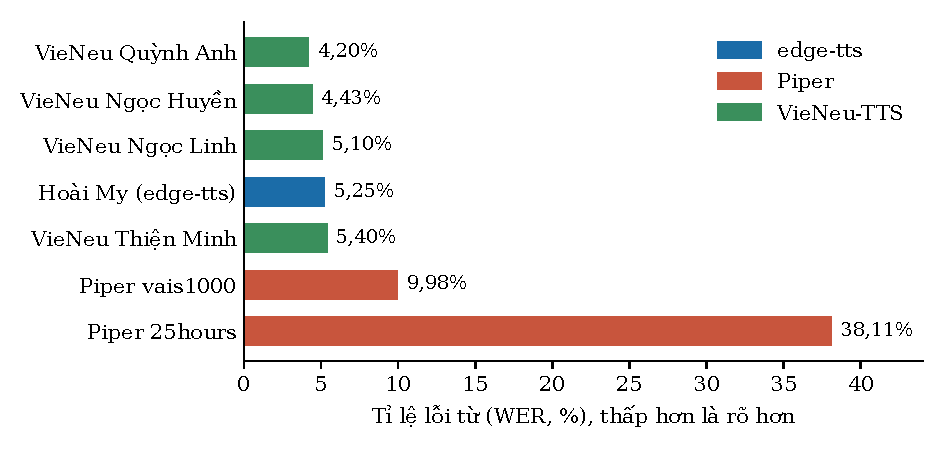
\includegraphics[width=0.82\textwidth]{bieu-do-wer.pdf}
\caption{Tỉ lệ lỗi từ của bảy cấu hình giọng, đo bằng cách cho mô hình nhận dạng tiếng nói nghe lại âm thanh tổng hợp.}
\label{fig:wer}
\end{figure}

\subsection{Ba phát hiện}\label{sec:phat-hien}

\begin{enumerate}
\def\labelenumi{\arabic{enumi}.}
\tightlist
\item
  \textbf{Một giọng Piper tiếng Việt không có thanh điệu.} Bảng ký hiệu âm vị của giọng \texttt{25hours\_single-low} thiếu các ký hiệu thanh điệu: 806 trên 8.068 âm vị của văn bản thử (10,0\%) bị bỏ khi đưa vào mô hình, và toàn bộ số bị bỏ là ký hiệu thanh. WER lên 38\%. Bài học: chọn giọng cho tiếng Việt phải kiểm tra bảng ký hiệu của mô hình, không chỉ nhìn tên ngôn ngữ.
\item
  \textbf{VieNeu-TTS chạy được trên CPU nhanh hơn thời gian thực}, đúng như dự án tự nhận, với độ rõ ngang giọng thương mại của Microsoft. Nhưng nó không tăng tốc được bằng cách chạy song song trên máy này: một tiến trình đạt RTF 0,74, hai tiến trình cùng lúc đạt RTF 1,74 mỗi tiến trình.
\item
  \textbf{WER không phản ánh hết chất lượng nghe.} Piper có WER gấp đôi nhưng lý do người nghe thử chê nó là ngữ điệu, điều WER không đo. Mục 5.1 phân tích tiếp.
\end{enumerate}

\subsection{Trang nghe thử}

Để chọn giọng bằng tai chứ không chỉ bằng số, chúng em dựng một trang nghe thử phát cùng các đoạn văn bằng từng giọng (\texttt{demo/make\_listen\_page.py}, đã đưa lên ở đường dẫn \texttt{/nghe-thu/} của trang sản phẩm). Người nghe ở đây mới là chính chúng em, chưa phải một nhóm người nghe chấm điểm mù.

\section{Ứng dụng Sách Nói}

\subsection{Kiến trúc}

\begin{figure}[H]
\centering
\begin{tikzpicture}[every node/.style={font=\small},
  b/.style={draw=accent, fill=boxfill, rounded corners=2pt, minimum height=9mm, text width=5.6cm, align=center},
  n/.style={text width=7.4cm, align=left, font=\footnotesize},
  >={Stealth[length=2.2mm]}]
\node[b] (a) at (0,0) {Wikisource\\ {\footnotesize tác phẩm thuộc phạm vi công cộng}};
\node[b] (b) at (0,-2.2) {Văn bản đã tách đoạn\\ {\footnotesize\texttt{segments.json}, \texttt{dtbook.xml}}};
\node[b] (c) at (0,-4.6) {Bộ DAISY 3 cho mỗi giọng đọc\\ {\footnotesize DTBook, SMIL, OPF, NCX, mp3}};
\node[b] (d) at (0,-6.8) {Trang tĩnh\\ {\footnotesize danh mục, dữ liệu JSON, âm thanh}};
\node[b] (e) at (0,-9.0) {Ứng dụng Sách Nói\\ {\footnotesize GitHub Pages, cài được lên điện thoại}};
\draw[->] (a) -- (b); \draw[->] (b) -- (c); \draw[->] (c) -- (d); \draw[->] (d) -- (e);
\node[n, anchor=west] at (3.3,-1.1) {\texttt{import\_wikisource.py}: lấy văn bản, tách đoạn, gán định danh, từ chối trang không có nhãn phạm vi công cộng};
\node[n, anchor=west] at (3.3,-3.4) {\texttt{tts\_chapter\_edge.py}: đọc từng đoạn, lấy mốc từng câu\\ \texttt{gen\_smil.py}, \texttt{gen\_opf\_ncx.py}: sinh bộ file DAISY\\ \texttt{validate\_daisy.py}: kiểm tra chéo};
\node[n, anchor=west] at (3.3,-5.7) {\texttt{build\_site.py}: lập danh mục và dữ liệu rút gọn cho ứng dụng};
\node[n, anchor=west] at (3.3,-7.9) {\texttt{deploy\_site.py}: đưa trang lên nơi lưu trữ};
\end{tikzpicture}
\caption{Dây chuyền từ văn bản trên Wikisource tới ứng dụng. Cột bên phải ghi script thực hiện từng bước.}
\label{fig:kien-truc}
\end{figure}

Ứng dụng là trang web tĩnh viết bằng HTML, CSS và JavaScript thuần (không dùng khung giao diện), cài được lên màn hình chính như một ứng dụng (PWA). Chúng em chọn web thay cho ứng dụng gốc vì ba lý do: chạy ngay trên mọi điện thoại không cần cài qua kho ứng dụng, triển khai bằng GitHub Pages không tốn chi phí máy chủ, và trình đọc màn hình của cả Android lẫn iOS đều hỗ trợ tốt nội dung web có đánh dấu ngữ nghĩa. Cái giá là không dùng được một số khả năng của hệ điều hành (ví dụ phím âm lượng làm cử chỉ).

\textbf{Cài lên điện thoại.} Có ba cách, đều ghi trong mục Cài ứng dụng của trang Hướng dẫn. Trên Android, người dùng tải file \texttt{SachNoi.apk} ngay từ trang; đây là bản đóng gói Trusted Web Activity dựng bằng Bubblewrap (\texttt{app/android}), nặng chưa tới 1 MB vì nó chỉ mở trang web trong Chrome ở chế độ toàn màn hình, nhờ vậy mọi cập nhật của trang có ngay trong ứng dụng mà không phải dựng lại APK. Cũng trên Android có thể chọn Thêm vào màn hình chính trong Chrome. Trên iPhone và iPad, người dùng mở trang bằng Safari rồi chọn Thêm vào Màn hình chính; chúng em chưa làm bản cài riêng cho iOS vì việc đó cần máy Mac và tài khoản Apple Developer. Hai giới hạn: APK còn hiện một thanh địa chỉ mỏng do chưa đặt được file \texttt{assetlinks.json} ở gốc tên miền, và chúng em chưa thử cách cài nào trên điện thoại thật.

Mỗi cuốn sách vẫn là một bộ DAISY 3 hợp lệ (DTBook, SMIL, OPF, NCX), mở được bằng phần mềm đọc DAISY khác. Ứng dụng đọc một bản rút gọn dạng JSON sinh từ chính bộ DAISY đó để tải nhanh trên điện thoại.

\subsection{Thư viện}

Thư viện gồm 15 đầu sách. Mười bốn cuốn chúng em dựng trong đồ án này có 115 phần, tổng cộng 974 phút âm thanh (khoảng 16 giờ), tất cả đã nghe được trên trang sản phẩm:

{\small
\begin{longtable}[]{@{}>{\raggedright\arraybackslash}p{2.8cm}>{\raggedright\arraybackslash}p{12.0cm}@{}}
\caption{Các đầu sách của thư viện theo thể loại}\label{tab:thu-vien}\\
\toprule\noalign{}
Thể loại & Sách \\
\midrule\noalign{}
\endhead
\bottomrule\noalign{}
\endlastfoot
Truyện ngắn & Lão Hạc, Chí Phèo (Nam Cao); Hai đứa trẻ, Gió lạnh đầu mùa, Cô hàng xén, Dưới bóng hoàng lan (Thạch Lam) \\
Tiểu thuyết & Tắt đèn (Ngô Tất Tố), 27 chương \\
Tùy bút & Hà Nội băm sáu phố phường (Thạch Lam), 21 bài \\
Thơ & Truyện Kiều (Nguyễn Du), 13 phần; Thơ Hàn Mặc Tử, 4 phần \\
Ngâm khúc & Chinh phụ ngâm (Đặng Trần Côn, bản diễn Nôm tương truyền của Đoàn Thị Điểm), 4 phần \\
Truyện truyền kỳ & Truyền kỳ mạn lục (Nguyễn Dữ, Ngô Văn Triện dịch), 20 truyện \\
Lịch sử & Việt Nam sử lược (Trần Trọng Kim), lời tựa và hai phần đầu, 12 mục \\
Khảo cứu & Việt Nam phong tục (Phan Kế Bính), 8 mục đầu \\
Thiếu nhi & Totto-chan bên cửa sổ, cuốn của đồ án giữa kỳ, mở bằng trình phát cũ \\
\end{longtable}
}

\textbf{Bản quyền.} Mười bốn cuốn mới đều lấy từ Wikisource tiếng Việt và thuộc phạm vi công cộng theo Luật Sở hữu trí tuệ (suốt đời tác giả cộng 50 năm). Bộ nhập sách từ chối trang không có nhãn phạm vi công cộng. Các tựa trong danh sách tài liệu của lớp còn bản quyền (Dế Mèn phiêu lưu ký, Vang bóng một thời...) và các truyện cổ tích không rõ nguồn bản kể không được đưa vào; căn cứ từng cuốn ghi ở \texttt{books/README.md}. Totto-chan còn bản quyền, nên chúng em chỉ giữ dưới dạng liên kết tới trang giữa kỳ đã nộp. Bìa sách dựng từ ảnh thuộc phạm vi công cộng hoặc giấy phép mở trên Wikimedia Commons, có ghi nguồn trong ứng dụng.

\textbf{Giới hạn dung lượng.} GitHub Pages giới hạn 1 GB; trang giữa kỳ đã chiếm 410 MB và bản hiện tại dùng 986 MB. Vì vậy Việt Nam sử lược và Việt Nam phong tục chỉ có phần đầu, và các sách dài thêm sau không kèm file zip DAISY tải về.

\subsection{Tính năng}

Chúng em lập danh sách tính năng bằng cách đối chiếu với những ứng dụng và máy đọc sách mà người khiếm thị đang dùng (BARD Mobile, Legimus, Voice Dream Reader, Victor Reader Stream, Dolphin EasyReader) cùng các tiêu chí của DAISY Consortium, rồi bổ sung dần những gì còn thiếu. Sau các lần đối chiếu, thứ các sản phẩm đó có mà Sách Nói chưa có là chỉnh âm sắc của giọng đọc. Hình~\ref{fig:man-hinh} cho thấy ba màn hình chính; phần còn lại của mục này mô tả tính năng theo bốn nhóm.

\begin{figure}[H]
\centering
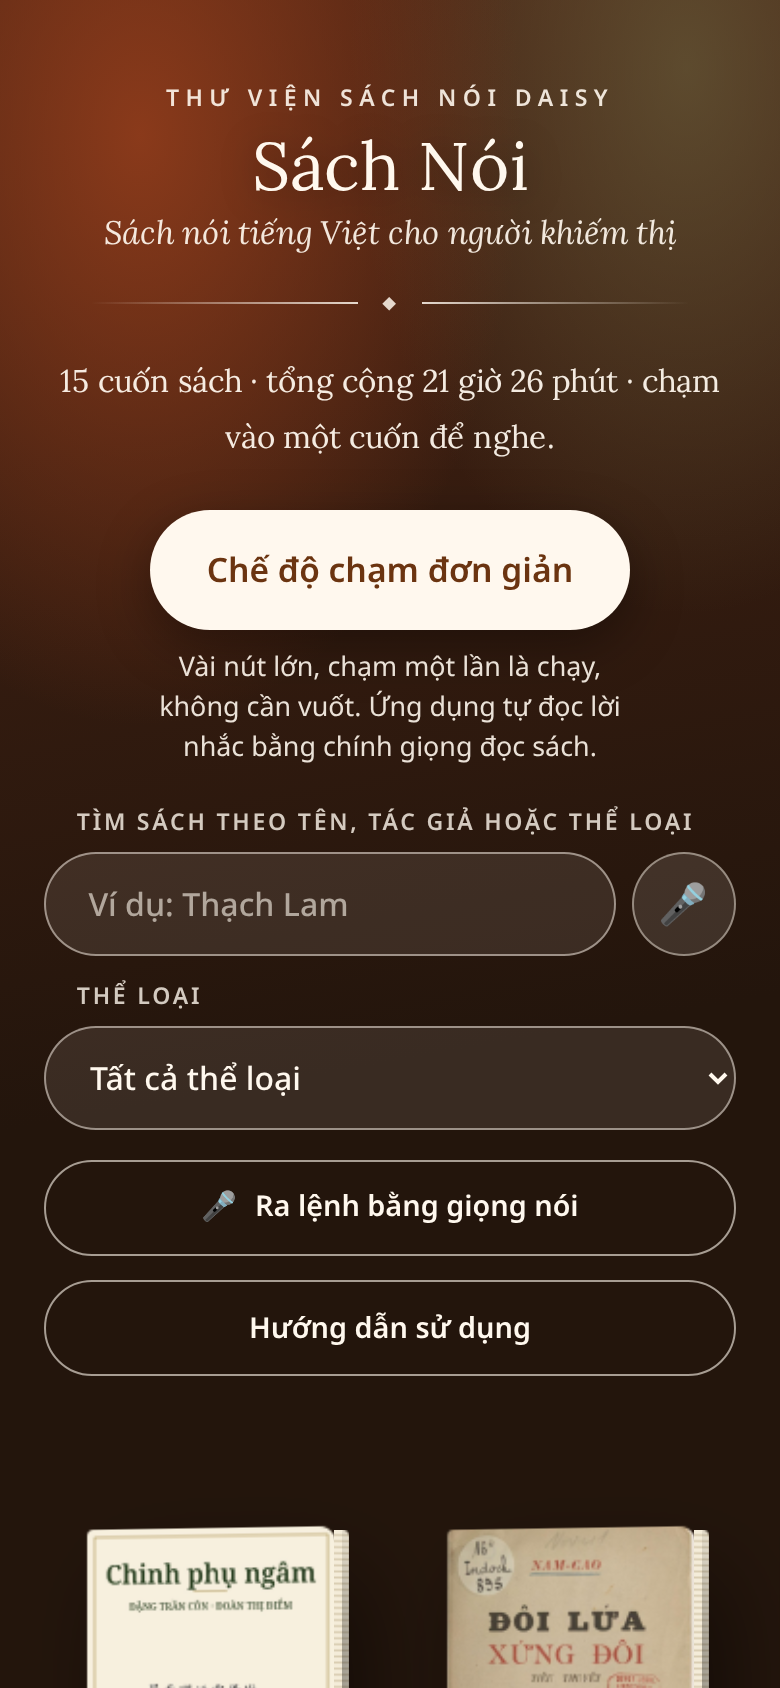
\includegraphics[width=0.31\textwidth]{app-thu-vien.png}\hfill
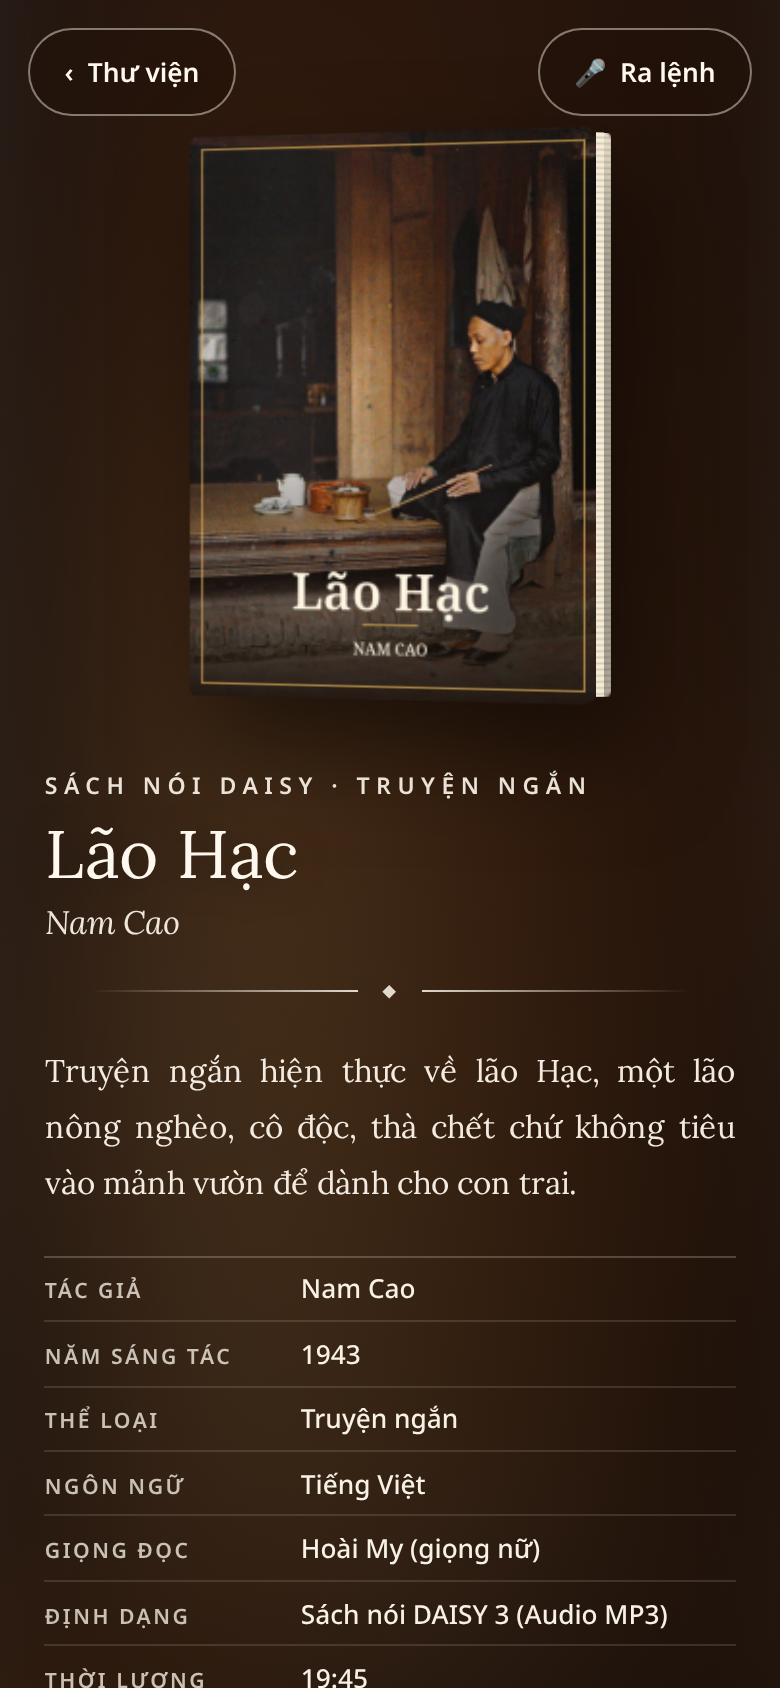
\includegraphics[width=0.31\textwidth]{app-trang-bia.png}\hfill
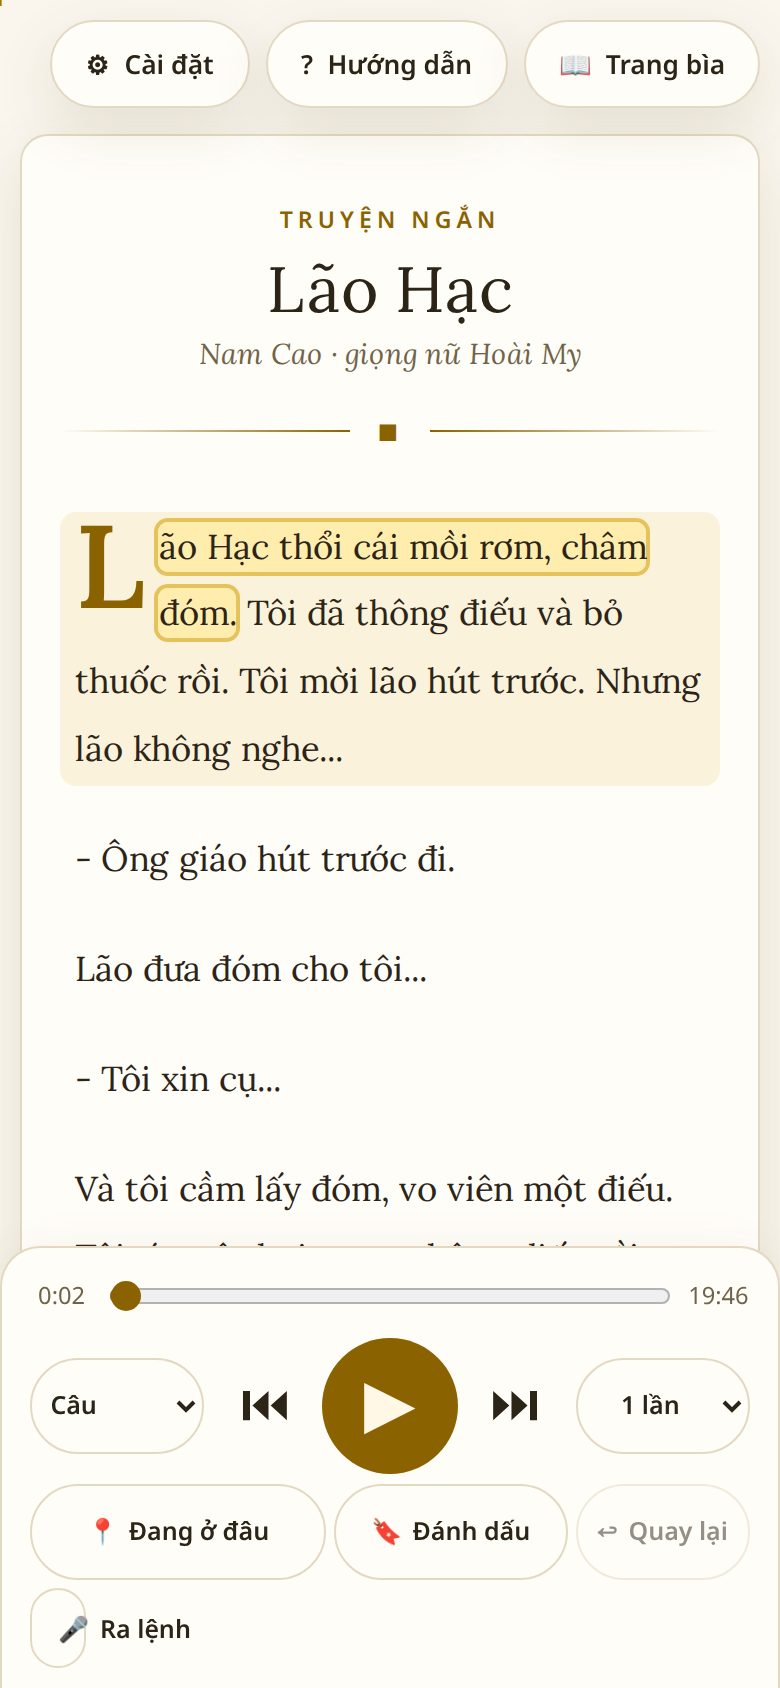
\includegraphics[width=0.31\textwidth]{app-trang-doc.png}
\caption{Ba màn hình chính của ứng dụng trên điện thoại: thư viện (trái), trang bìa của một cuốn sách (giữa) và trang đọc với câu đang đọc được tô sáng (phải).}
\label{fig:man-hinh}
\end{figure}

\subsubsection{Nghe và điều hướng}

Trên trang đọc, văn bản hiện cùng âm thanh và câu đang đọc được tô sáng; chạm vào câu nào thì ứng dụng đọc từ câu đó. Việc di chuyển trong sách dựa trên một cặp nút lùi và tới duy nhất, đi kèm một \textbf{bước nhảy do người nghe chọn}: câu, đoạn, 30 giây, phần hoặc dấu trang. Các máy đọc sách cho người mù như Victor Reader Stream tổ chức điều hướng theo đúng cách này, vì nó giữ số nút ở mức ít nhất mà vẫn đi được tới mọi chỗ trong sách. Nếu nhảy nhầm, nút \textbf{Quay lại} hủy cú nhảy vừa rồi, kể cả khi người nghe đã sang phần khác.

Tốc độ đọc chỉnh được từ 0,5 đến 3 lần và được nhớ riêng cho từng cuốn, vì người dùng trình đọc màn hình lâu năm thường nghe ở tốc độ rất cao. Ứng dụng nhớ vị trí đang nghe của từng cuốn, đưa cuốn nghe dở lên mục Nghe tiếp ở đầu thư viện và tự chuyển sang phần sau khi hết một phần. Người nghe có thể đánh dấu trang, kèm một ghi chú thu bằng giọng nói của chính mình, và hẹn giờ tắt theo số phút hoặc khi hết phần.

Hai tính năng sau tận dụng trực tiếp mốc thời gian của từng câu. Thứ nhất là \textbf{lùi về đầu câu khi nghe tiếp}: sau khi dừng hơn 20 giây hoặc khi mở lại sách, ứng dụng phát lại từ đầu câu đang nghe dở để người nghe bắt lại mạch, và nếu câu đó mới nghe chưa tới 2 giây thì lùi thêm một câu. BARD Mobile cũng lùi lại khi nghe tiếp nhưng lùi theo một số giây cố định, nên có thể rơi vào giữa câu. Tính năng này tắt được trong phần Cài đặt. Thứ hai là \textbf{tìm trong sách}: ở trang bìa, người dùng gõ một từ hoặc một câu, không cần gõ dấu; ứng dụng tìm trong văn bản của mọi phần, báo số câu tìm thấy bằng lời và mở đúng câu được chọn.

\subsubsection{Dùng không cần nhìn}

Mọi nút đều có nhãn bằng lời. Mọi thay đổi trạng thái, chẳng hạn đổi bước nhảy, tới đầu hoặc cuối sách, hay vừa đánh dấu trang, đều được báo qua vùng thông báo dành cho trình đọc màn hình, kèm một tiếng báo hiệu ngắn có thể tắt. Thứ tự đọc của trang đặt các nút điều khiển trước nội dung sách, để người dùng trình đọc màn hình không phải vuốt qua cả chương mới tới được nút phát. Nút \textbf{Đang ở đâu} đọc tên sách, tên phần, thời điểm, thời gian còn lại và tốc độ, đáp ứng nhu cầu xác nhận vị trí trước khi nghe dài mà bài @BENCH nêu ra. Khi đang tạm dừng mà nhảy câu, ứng dụng đọc ngay câu đó, nhờ vậy người nghe dò được từng câu một. Mọi thao tác đều có phím tắt và ứng dụng có sẵn một trang hướng dẫn. Sách tìm được bằng cách gõ tên, tác giả, thể loại, hoặc bằng giọng nói nếu trình duyệt hỗ trợ nhận dạng tiếng nói.

\paragraph{Chế độ chạm đơn giản.} Trình đọc màn hình buộc người dùng vuốt qua từng phần tử rồi nhấp đôi, nên một trang nhiều nút rất tốn thao tác. Chế độ chạm đơn giản (Hình~\ref{fig:don-gian}) thay cả màn hình bằng vài nút rất lớn ở vị trí cố định: nhắc lại và hướng dẫn, lùi, tới, nghe hoặc tạm dừng, đổi sách. Chạm một lần là chạy, không cuộn và không vuốt. Khi đang nghe, màn hình có thêm một nút đổi chức năng của hai nút lùi và tới giữa năm mức: 30 giây, chọn phần, đổi tốc độ, dấu trang (đánh dấu và đi tới dấu trang) và hẹn giờ tắt. Đây cũng là cách máy Victor Reader giữ ít phím mà vẫn đủ việc.

Trong chế độ này ứng dụng tự đọc lời nhắc và hướng dẫn, đồng thời vặn nhỏ tiếng sách trong lúc đọc, nên dùng được cả khi không bật trình đọc màn hình. Bản đầu tiên dùng giọng tiếng Việt có sẵn của máy qua Web Speech API. Cách đó hỏng trên những máy không cài giọng tiếng Việt, vì trình duyệt sẽ đọc chữ Việt bằng giọng tiếng Anh. Vì vậy chúng em viết lại mọi lời nhắc thành các câu ngắn chỉ lấy giá trị từ những tập đếm được (tên sách, tên phần, số phút, tốc độ), tổng cộng khoảng 1.200 câu. Các câu này được thu sẵn bằng chính giọng Hoài My của thư viện (\texttt{pipeline/scripts/build\_prompts.py}) và phát nối nhau khi cần. Câu nào không có bản thu thì ứng dụng mới dùng giọng của máy, và nếu máy không có giọng tiếng Việt thì lời nhắc hiện bằng chữ.

\begin{figure}[H]
\centering
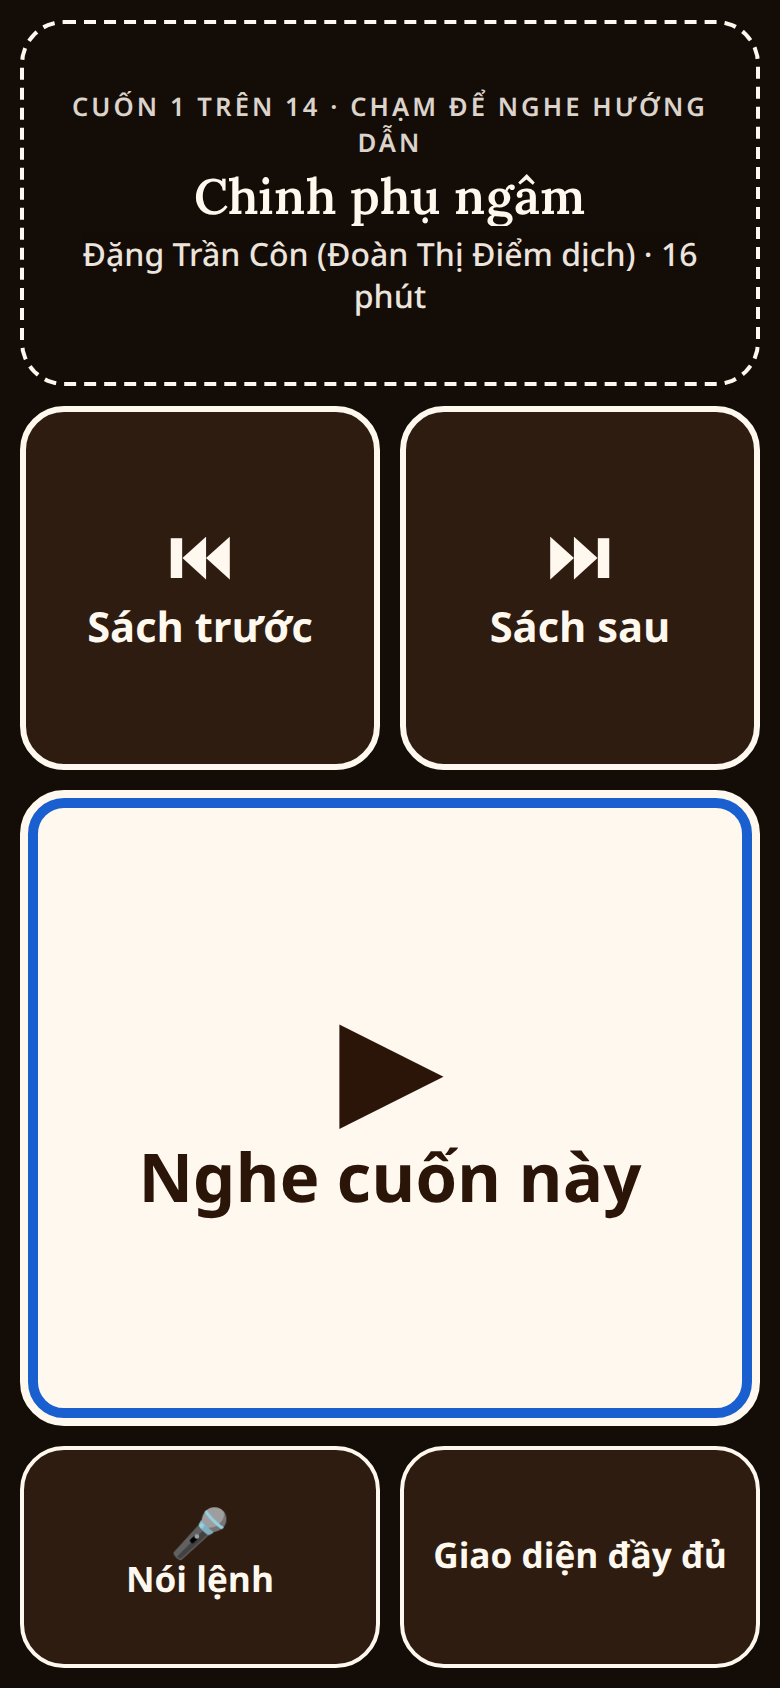
\includegraphics[width=0.31\textwidth]{app-don-gian-chon.png}\hfill
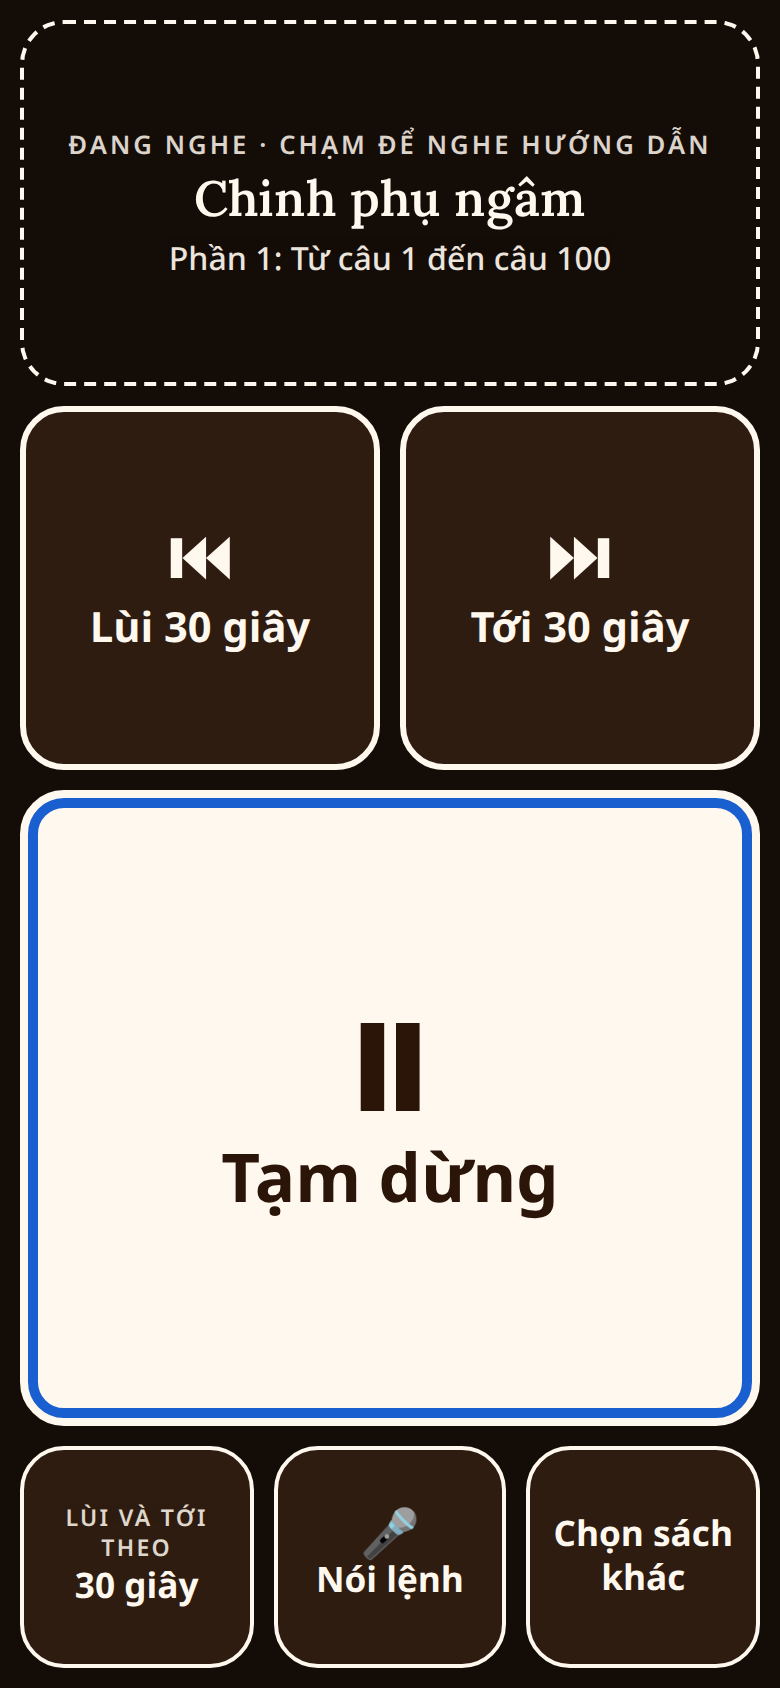
\includegraphics[width=0.31\textwidth]{app-don-gian-nghe.png}\hfill
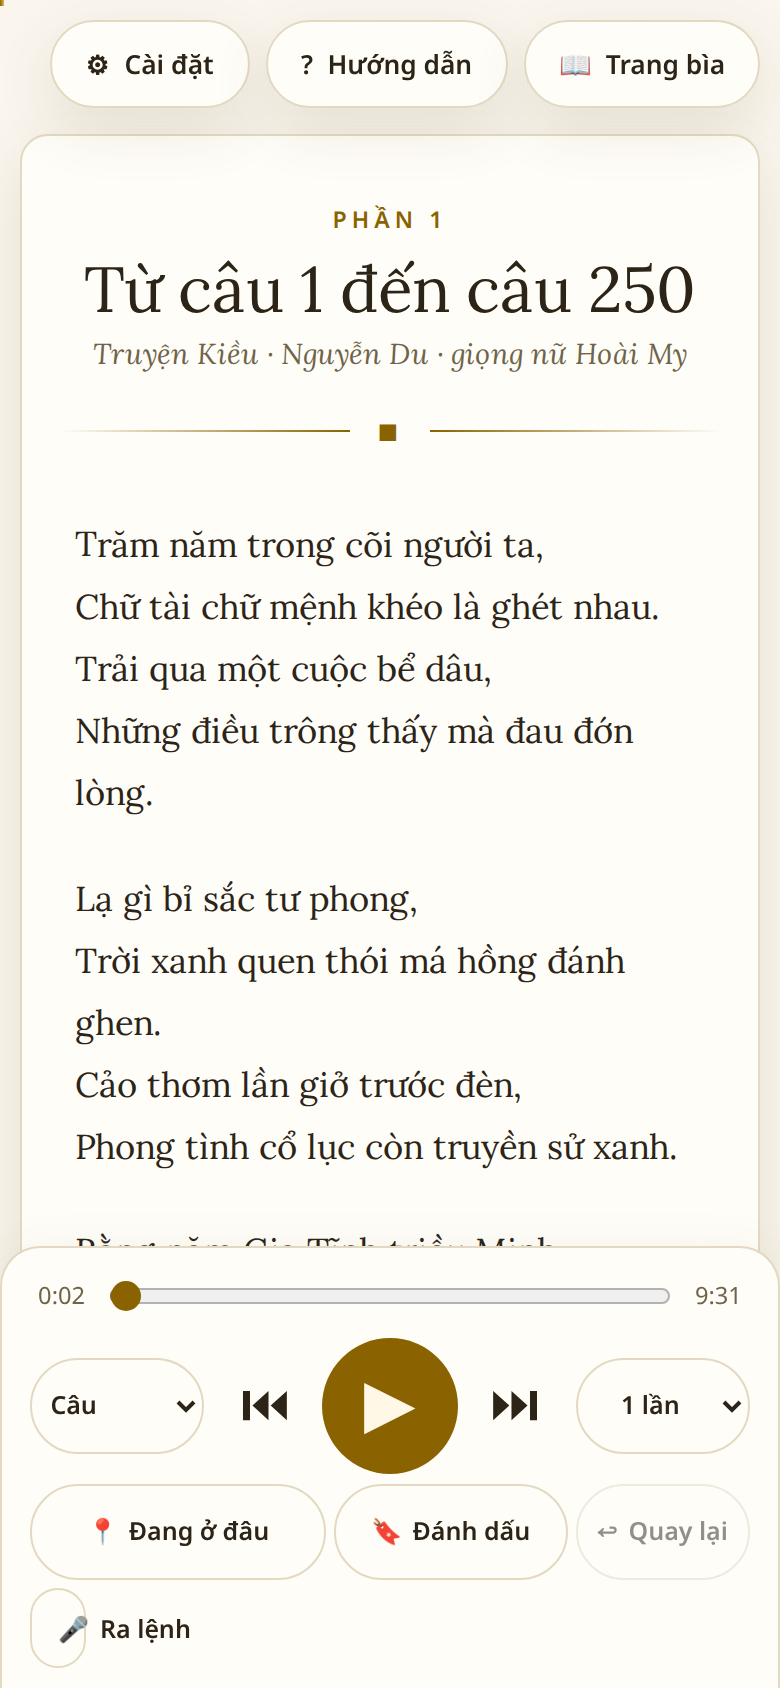
\includegraphics[width=0.31\textwidth]{app-tho.png}
\caption{Chế độ chạm đơn giản lúc chọn sách (trái) và lúc đang nghe (giữa); trang đọc của Truyện Kiều với mỗi câu thơ trên một dòng (phải).}
\label{fig:don-gian}
\end{figure}

\paragraph{Điều khiển bằng giọng nói.} Người dùng bấm nút micro một lần, nghe tiếng báo rồi nói một lệnh tiếng Việt: phát, tạm dừng, lùi hoặc tới kèm số giây hay số phút, câu trước, câu sau, phần trước, phần sau, phần số mấy, nhanh hơn, chậm hơn, đánh dấu, tới dấu trang, hẹn giờ kèm số phút, đang ở đâu, thư viện, hoặc mở kèm tên sách hay tên tác giả. Ứng dụng dùng bộ nhận dạng tiếng nói của trình duyệt (Web Speech API, \texttt{vi-VN}) rồi tự hiểu lệnh bằng luật. Từ khoá được so khớp trên câu đã bỏ dấu để chịu được lỗi dấu của bộ nhận dạng, nhưng con số được đọc trên câu còn dấu để phân biệt ``phần sáu'' với ``phần sau''. Chúng em chọn cách bấm rồi nói thay vì luôn lắng nghe, vì micro luôn mở sẽ thu lẫn tiếng sách; trong lúc nghe lệnh, sách tạm dừng rồi tự phát tiếp. Nút micro có ở giao diện đầy đủ lẫn hàng dưới cùng của chế độ chạm đơn giản, nơi câu trả lời được phát bằng bản thu sẵn giọng Hoài My. Tính năng này cần mạng và chỉ hiện khi trình duyệt hỗ trợ.

\subsubsection{Dùng với thị lực kém}

Người còn một phần thị lực chọn được một trong ba nền (giấy, tối, tương phản cao), bốn cỡ chữ và một kiểu chữ dễ đọc. Câu đang đọc có thể được tô bằng một trong ba màu, gạch chân, hoặc không đánh dấu. Mọi vùng chạm rộng ít nhất 44 điểm ảnh và bố cục đã được kiểm tra tới màn hình rộng 320 điểm ảnh.

\subsubsection{Trên điện thoại}

Ứng dụng điều khiển được từ màn hình khóa và từ tai nghe qua Media Session, có hiện ảnh bìa. Từng cuốn sách lưu được vào máy để nghe khi mất mạng (âm thanh nằm trong IndexedDB), và ứng dụng cài được lên màn hình chính như mô tả ở mục 4.1.

\paragraph{Thơ hiện theo từng dòng thơ.} Lúc nhập văn bản, các dòng thơ được nối thành đoạn để giọng đọc đọc liền mạch, nên trang đọc từng hiện thơ như văn xuôi. Để sửa, \texttt{pipeline/scripts/verse\_lines.py} lấy lại từng dòng thơ từ Wikisource; khi lắp trang, \texttt{build\_site.py} so khớp các dòng đó với văn bản từng câu và chỉ ghi thêm vị trí cần xuống dòng. Chữ, âm thanh và mốc thời gian không đổi nên không phải thu lại. Truyện Kiều (820 đoạn) và Chinh phụ ngâm (103 đoạn) khớp toàn bộ; Thơ Hàn Mặc Tử khớp 68 trên 80 đoạn, 12 đoạn còn lại là thơ văn xuôi vốn không ngắt dòng. Ảnh bên phải của Hình~\ref{fig:don-gian} cho thấy kết quả.

\paragraph{Nhập sách của riêng người dùng.} Ở cuối thư viện, người dùng chọn một file zip chứa sách nói DAISY 2.02 hoặc DAISY 3 có sẵn trên máy. Ứng dụng đọc file ngay trong trình duyệt (\texttt{app/web/daisy-import.js}) và không gửi gì lên mạng. Nó đọc mục lục của file zip rồi chỉ cắt từng file con khi cần, để một cuốn sách vài trăm MB không phải nạp cả vào bộ nhớ. Thứ tự đọc được lấy từ OPF hoặc \texttt{ncc.html}, mốc thời gian lấy từ SMIL, văn bản lấy từ DTBook hoặc HTML; sau đó mỗi file âm thanh được lưu thành một phần trong IndexedDB theo đúng dạng của sách lưu ngoại tuyến. Nhờ vậy trang đọc được dùng lại nguyên vẹn: sách có văn bản thì được tô sáng theo lời đọc, còn sách chỉ có tiếng vẫn tua, đánh dấu, chọn phần và hẹn giờ như thường. Chúng em đã thử bộ đọc với bốn cuốn mẫu của DAISY Consortium (hai cuốn 2.02 chỉ có mục lục, một cuốn 2.02 đủ văn bản, một cuốn DAISY 3) và với các file do chính dây chuyền của nhóm sinh ra.

\subsection{Kiểm thử}

\begin{itemize}
\tightlist
\item
  \textbf{Cấu trúc DAISY:} \texttt{validate\_daisy.py} kiểm tra chéo cho từng phần của từng cuốn: mọi đoạn trong DTBook có mốc trong SMIL, mốc thời gian tăng dần và nằm trong thời lượng file âm thanh, OPF và NCX khớp nhau. Mọi phần đã dựng đều qua.
\item
  \textbf{Giao diện:} 178 kiểm thử đầu-cuối chạy trên Chromium qua Playwright ở kích thước màn hình điện thoại (\texttt{app/tests/e2e.py}). Chúng kiểm tra hành vi thật chứ không chỉ sự tồn tại của nút: ví dụ nhảy 30 giây thì thời điểm phát tăng trong khoảng 29,5 đến 32 giây; chọn thể loại "Thơ" thì thư viện chỉ còn đúng các tập thơ; ghi âm ghi chú bằng micro giả rồi kiểm tra dữ liệu âm thanh đã nằm trong bộ nhớ của máy.
\item
  \textbf{Giới hạn của kiểm thử tự động:} nó xác nhận nhãn, vai trò, thứ tự và thông báo có mặt trong trang, không xác nhận TalkBack hay VoiceOver đọc chúng ra sao. Việc này chúng em chưa làm được (mục 6).
\end{itemize}

\section{Phân tích sâu: chọn và cải tiến bước TTS cho sách nói tiếng Việt}

Chúng em chọn bước tổng hợp tiếng nói để phân tích sâu, vì nó quyết định cả chất lượng nghe lẫn khả năng mở rộng thư viện. Chỉ trong hai tuần, chúng em đã đổi giọng đọc của thư viện ba lần, và lần nào cũng có số liệu và lý do đi kèm.

\subsection{Vì sao giọng nhanh nhất không dùng được: phép đo mà WER bỏ sót}

Lựa chọn đầu tiên của chúng em là Piper: chạy trên CPU nhanh gấp 27--40 lần thời gian thực, không phụ thuộc mạng, WER 10\%. Cả thư viện dựng xong trong vài phút. Nhưng khi nghe thử, chúng em thấy ngữ điệu kém giọng Hoài My của bản giữa kỳ rõ rệt, điều mà WER (chỉ đo từng từ có nghe ra hay không) không thể hiện.

Hai phép đo bổ sung trên cùng 20 đoạn cho kết quả ở Bảng~\ref{tab:nhip} và Hình~\ref{fig:nhip}.

{\small
\begin{longtable}[]{@{}>{\raggedright\arraybackslash}p{3.6cm}>{\raggedright\arraybackslash}p{3.2cm}>{\raggedright\arraybackslash}p{3.6cm}>{\raggedright\arraybackslash}p{3.6cm}@{}}
\caption{Tốc độ đọc và tỉ lệ khoảng lặng của bốn giọng trên cùng 20 đoạn văn}\label{tab:nhip}\\
\toprule\noalign{}
Giọng & Tốc độ đọc (âm tiết/phút) & Tốc độ lúc đang phát âm & Phần thời gian là khoảng lặng \\
\midrule\noalign{}
\endhead
\bottomrule\noalign{}
\endlastfoot
Hoài My (edge-tts) & 186 & 286 & 34,8\% \\
Piper vais1000 & 275 & 295 & 6,7\% \\
VieNeu Ngọc Linh & 241 & 284 & 15,1\% \\
VieNeu Thiện Minh & 254 & 321 & 20,7\% \\
\end{longtable}
}

Lúc đang phát âm, các giọng nói nhanh gần như nhau (284--321 âm tiết mỗi phút). Khác biệt nằm ở khoảng lặng: Piper \textbf{gần như không ngắt nghỉ} (6,7\% thời gian), còn Hoài My dành hơn một phần ba thời gian cho chỗ nghỉ. Chúng em cho rằng lý do là mô hình VITS nhỏ, huấn luyện trên khoảng một nghìn câu đọc rời, không học được chỗ nghỉ ở dấu phẩy và giữa các ý. Với sách nói, chỗ nghỉ là lúc người nghe kịp hiểu; tốc độ đọc của Piper cũng cao hơn nhiều so với mốc 201 của bộ sách nói PhoAudiobook.

Khoảng lặng được tính bằng ngưỡng năng lượng đơn giản (khung 20 ms có RMS dưới 1\% mức đỉnh) nên chỉ dùng để so tương đối; file của edge-tts còn có khoảng lặng đệm ở hai đầu mỗi đoạn.

\begin{figure}[H]
\centering
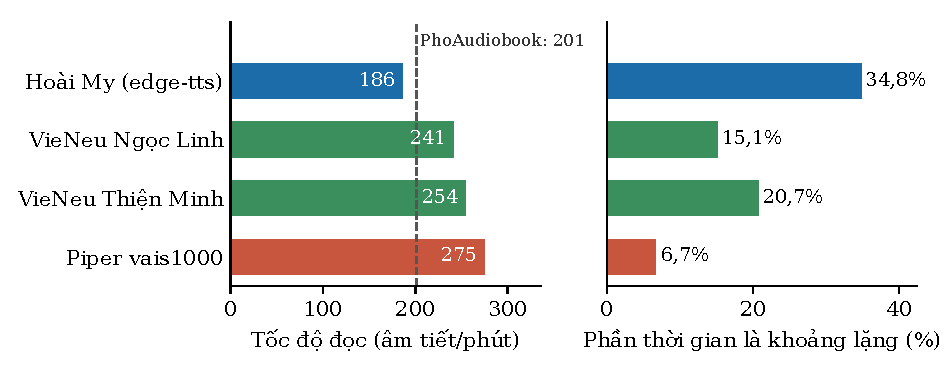
\includegraphics[width=0.9\textwidth]{bieu-do-nhip-doc.pdf}
\caption{Tốc độ đọc và tỉ lệ khoảng lặng của bốn giọng. Đường đứt nét là tốc độ đọc trung bình của bộ sách nói PhoAudiobook (201 âm tiết mỗi phút).}
\label{fig:nhip}
\end{figure}

\subsection{Lỗi của Piper nằm ở đâu}

Chúng em xem lại 113 cặp từ mà mô hình nhận dạng nghe khác văn bản gốc trên audio của Piper:

\begin{itemize}
\tightlist
\item
  25 cặp (22\%) \textbf{chỉ khác thanh điệu}: "vả" thành "và", "mồi" thành "môi". Đây là điểm yếu thật của giọng đọc và là loại lỗi làm sai nghĩa trong tiếng Việt.
\item
  Nhầm phụ âm cuối và phụ âm đầu: "hạc" thành "hạt", "gắp" thành "gắt".
\item
  8 cặp không phải lỗi phát âm mà là mô hình nhận dạng viết "ba" thành "3"; các cặp này cũng xuất hiện với Hoài My, nên WER thật của mọi giọng thấp hơn bảng một chút.
\end{itemize}

\subsection{Cải tiến thứ nhất: VieNeu-TTS và lưới an toàn bắt câu đọc sót}

VieNeu-TTS giải quyết được vấn đề ngữ điệu (khoảng lặng 15--21\%, WER 4,2--5,4\%) mà vẫn chạy trên CPU. Cái giá:

\begin{itemize}
\tightlist
\item
  Chậm hơn Piper 20--40 lần: dựng hai giọng cho thư viện khi đó (khoảng 3,6 giờ audio mỗi giọng) mất nhiều giờ. Chúng em chuyển việc dựng thành hàng đợi chạy tiếp được sau khi ngắt và đưa lên trang dần theo từng phần (\texttt{build\_voices.py}).
\item
  \textbf{Có thể đọc sót.} Là mô hình tự hồi quy sinh mẫu ngẫu nhiên, nó đôi khi bỏ mất vài từ; trong 20 đoạn thử, giọng Thiện Minh bỏ một cụm ở một câu. Với người nghe khiếm thị, đây là lỗi nghiêm trọng vì họ không đối chiếu được bằng mắt.
\end{itemize}

Cách phát hiện chuẩn là cho mô hình nhận dạng nghe lại từng câu, nhưng việc đó làm thời gian dựng tăng gần gấp đôi. Chúng em đề xuất và cài đặt một \textbf{lưới an toàn theo nhịp đọc}, không tốn thêm thời gian: tính số giây mỗi âm tiết của từng câu; câu nào lệch khỏi trung vị của chương quá khoảng 0,65 đến 1,6 lần thì sinh lại. Khi đo trên một truyện thật, mọi câu bình thường nằm trong khoảng 0,8 đến 1,3 lần, nên ngưỡng này không bắt nhầm. Phương án kiểm tra bằng nhận dạng tiếng nói vẫn có sẵn qua tùy chọn \texttt{-\/-verify}.

\textbf{Giới hạn:} chúng em chưa đo tỉ lệ đọc sót trước và sau khi có lưới an toàn trên cả một cuốn sách, nên hiệu quả của lưới mới được kiểm trên các trường hợp đã biết.

\subsection{Cải tiến thứ hai: giọng dịch vụ với mốc câu lấy từ mốc từ}

Sau khi nghe cả thư viện bằng hai giọng VieNeu, cuối cùng (16/11) chúng em vẫn quay về giọng Hoài My vì ngữ điệu. Số liệu không phản bác lựa chọn này: Hoài My có WER ngang VieNeu và là giọng ngắt nghỉ nhiều nhất. Trở ngại trước đó của edge-tts là độ tin cậy và việc mất đồng bộ mức câu, không phải chất lượng. Chúng em gỡ hai trở ngại đó như sau.

\textbf{Giữ đồng bộ mức câu mà không cần mô hình căn chỉnh.} Bản giữa kỳ gửi cả đoạn văn cho dịch vụ và chỉ có mốc mức đoạn. Cách dễ nhất để có mốc câu là gửi từng câu, nhưng như vậy số yêu cầu tăng khoảng 5 lần và ngữ điệu liên câu bị mất. Cách chúng em cài đặt (\texttt{tts\_chapter\_edge.py}): vẫn gửi cả đoạn, yêu cầu dịch vụ trả về sự kiện mốc từng từ (WordBoundary), rồi gán lần lượt các từ vào các câu theo số từ của mỗi câu để ra mốc đầu và mốc cuối của câu. Hai cách tách từ (của dịch vụ và của dây chuyền) được so khớp; nếu không khớp thì đoạn đó lùi về chia thời lượng theo số ký tự. Trong lần dựng Chí Phèo, 5 trên 150 đoạn phải lùi về cách này.

Cùng cơ chế đếm từ đó phát hiện được \textbf{audio bị cụt}: dịch vụ đôi khi trả về âm thanh thiếu vài từ cuối. Nếu số từ nhận về ít hơn số từ gửi đi thì đoạn được tải lại.

\textbf{Tăng độ bền khi gọi dịch vụ.} Theo số đo của chúng em ngày 18/11, mỗi lần gọi hỏng với xác suất khoảng ba phần tư, bất kể đã chờ bao lâu giữa hai lần gọi. Vì vậy chiến lược chờ lâu dần của bản trước chỉ làm chậm. Ba thay đổi sau được áp dụng (Bảng~\ref{tab:do-ben}):

{\small
\begin{longtable}[]{@{}>{\raggedright\arraybackslash}p{7.2cm}>{\raggedright\arraybackslash}p{7.6cm}@{}}
\caption{Ba thay đổi làm tăng độ bền khi gọi dịch vụ và kết quả đo được}\label{tab:do-ben}\\
\toprule\noalign{}
Thay đổi & Kết quả đo \\
\midrule\noalign{}
\endhead
\bottomrule\noalign{}
\endlastfoot
Thử lại sau 0,5 giây thay cho chờ lâu dần; tải nhiều đoạn cùng lúc & Từ 1,4 lên khoảng 12 đoạn mỗi phút khi tải 4 đoạn cùng lúc, 18 đoạn mỗi phút khi tải 8 \\
Giới hạn thời gian cho mỗi yêu cầu & Hết hiện tượng một kết nối treo im lặng hàng chục phút \\
Đoạn hỏng 10 lần liên tiếp thì chia đôi theo ranh giới câu, tải từng nửa rồi ghép, cộng dồn mốc thời gian & Một đoạn 2.365 ký tự của Chí Phèo bị từ chối suốt hơn một giờ đã dựng được; mốc câu qua chỗ ghép vẫn liền mạch \\
\end{longtable}
}

\textbf{Cái giá còn lại:} bước dựng phụ thuộc một dịch vụ không chính thức, không có cam kết. Người nghe không bị ảnh hưởng vì âm thanh được dựng sẵn; chúng em giữ hai bản VieNeu làm đường lùi, và ứng dụng tự phát giọng dự phòng (kèm lời báo) cho phần chưa có giọng chính.

\needspace{10\baselineskip}
\subsection{So sánh ba phương án}

{\small
\begin{longtable}[]{@{}>{\raggedright\arraybackslash}p{3.6cm}>{\raggedright\arraybackslash}p{3.4cm}>{\raggedright\arraybackslash}p{3.4cm}>{\raggedright\arraybackslash}p{3.8cm}@{}}
\caption{So sánh ba phương án TTS theo các tiêu chí của sách nói}\label{tab:ba-phuong-an}\\
\toprule\noalign{}
Tiêu chí & Piper & VieNeu-TTS & Hoài My (edge-tts) \\
\midrule\noalign{}
\endhead
\bottomrule\noalign{}
\endlastfoot
WER trên văn bản thử & 9,98\% & 4,2--5,4\% & 5,25\% \\
Khoảng lặng & 6,7\% & 15--21\% & 34,8\% \\
Tốc độ dựng & Gấp 27--40 lần thời gian thực & Gấp 1,1--1,6 lần & Phụ thuộc dịch vụ \\
Cần mạng khi dựng & Không & Không & Có \\
Nguy cơ sai nội dung & Sai thanh điệu & Đọc sót từ & Audio cụt (đã có kiểm tra) \\
Kích thước mô hình & 63 MB & 541 MB & Không áp dụng \\
Vai trò hiện tại & Giọng dự phòng & Giọng dự phòng, đối chứng & Giọng của thư viện \\
\end{longtable}
}

Điều chúng em rút ra từ phần phân tích: với sách nói, tiêu chí xếp hạng các hệ TTS không phải chỉ là WER và tốc độ như trong các bài báo đã đọc. Ngắt nghỉ và độ an toàn nội dung (không sót, không cụt) quan trọng ngang độ rõ, và cả hai đo được bằng công cụ rẻ: tỉ lệ khoảng lặng, nhịp đọc theo âm tiết, và phép đếm từ.

\subsection{Đề xuất cải tiến chưa thực hiện}

\begin{enumerate}
\def\labelenumi{\arabic{enumi}.}
\tightlist
\item
  \textbf{Chuẩn hóa văn bản trước TTS.} Số La Mã, ngày tháng, chữ viết tắt và lối viết gạch nối kiểu cũ ("Hồng-bàng") hiện được đọc nguyên trạng. Cần một bộ luật chuẩn hóa và phép đo WER trước, sau trên các câu có số.
\item
  \textbf{Thơ.} Thơ lục bát và song thất lục bát được ghép bốn câu thành một đoạn khi đưa cho giọng đọc. Trang đọc đã hiện lại từng dòng thơ (mục 4.3), nhưng chưa thử thêm chỗ nghỉ ở cuối mỗi câu thơ trong âm thanh.
\item
  \textbf{Điểm nghe chủ quan.} Chưa có phép chấm mù (MOS) với nhiều người nghe; lựa chọn giọng hiện dựa trên số đo khách quan và tai của chính nhóm.
\item
  \textbf{Câu thoại rất ngắn} ("Vâng!", "Này!") chỉ dài khoảng 0,2 giây với Piper, nghe cụt; hiện tượng cùng loại với lỗi câu ngắn mà PhoAudiobook báo cáo ở XTTS-v2.
\item
  \textbf{F5-TTS tiếng Việt} chúng em chưa so sánh được vì cần GPU.
\end{enumerate}

\section{Hạn chế}

\begin{itemize}
\tightlist
\item
  \textbf{Chúng em chưa thử với người khiếm thị}, và chưa thử trên điện thoại thật với TalkBack hoặc VoiceOver. Mọi kiểm tra trợ năng đến nay là kiểm thử tự động trên Chromium ở kích thước màn hình điện thoại. Đây là hạn chế lớn nhất của đồ án, và là việc chúng em muốn làm đầu tiên nếu có thêm thời gian.
\item
  Nhập sách chỉ nhận file zip DAISY có âm thanh; chưa đọc EPUB, sách DAISY chỉ có văn bản, sách có mã hoá bảo vệ và file zip trên 4 GB. Tên của sách tự nhập không có bản thu giọng Hoài My nên trong chế độ chạm đơn giản được đọc bằng giọng của máy hoặc hiện bằng chữ. Chưa thử với sách của các thư viện sách nói trong nước.
\item
  Micro thật và nhận dạng tiếng nói thật (cho tìm kiếm, ra lệnh và ghi chú bằng giọng nói) chúng em chưa thử được; kiểm thử dùng thiết bị giả và đưa thẳng câu chữ vào bộ hiểu lệnh. Vì vậy chưa biết tỉ lệ nhận đúng lệnh khi người thật nói, nhất là trong môi trường ồn hoặc với giọng địa phương.
\item
  Chúng em chưa nghe kiểm tra giọng Hoài My trên các thể loại mới thêm (thơ, văn bản có nhiều từ Hán Việt gạch nối).
\item
  Phép đo TTS chỉ trên một văn bản (20 đoạn của một truyện), một lần chạy cho mỗi giọng.
\item
  Chữ Hán, chữ Nôm và chú thích trong Truyền kỳ mạn lục, Việt Nam sử lược bị lược bỏ khi nhập; vài chỗ còn lỗi chính tả của bản số hóa trên Wikisource.
\item
  Thư viện bị chặn bởi giới hạn 1 GB của nơi lưu trữ.
\end{itemize}

\section{Kết luận}

Chúng em đã nối tiếp đồ án giữa kỳ thành một dây chuyền hoàn chỉnh từ văn bản thuộc phạm vi công cộng tới sách nói DAISY nghe được trên điện thoại, và cho thấy bằng số liệu rằng việc chọn hệ TTS cho sách nói cần những phép đo ngoài WER. Ứng dụng đã chạy công khai với 15 đầu sách và đã có bộ kiểm thử tự động; bước còn thiếu để gọi nó là dùng được cho người khiếm thị là thử nghiệm với chính họ.

\begin{thebibliography}{99}
\addcontentsline{toc}{section}{Tài liệu tham khảo}
\setlength{\itemsep}{2pt}
\bibitem{b1} Thi Vu, Linh The Nguyen, Dat Quoc Nguyen. Zero-Shot Text-to-Speech for Vietnamese. ACL 2025 (Short Papers), tr. 1042--1049.
\bibitem{b2} Yushen Chen, Zhikang Niu, Ziyang Ma, Keqi Deng, Chunhui Wang, Jian Zhao, Kai Yu, Xie Chen. F5-TTS: A Fairytaler that Fakes Fluent and Faithful Speech with Flow Matching. ACL 2025 (Long Papers), tr. 6255--6271.
\bibitem{b3} Shengpeng Ji và cộng sự. MobileSpeech: A Fast and High-Fidelity Framework for Mobile Zero-Shot Text-to-Speech. ACL 2024 (Long Papers).
\bibitem{b4} Xin Jiang, Junwei Zheng, Ruiping Liu, Jiahang Li, Jiaming Zhang, Sven Matthiesen, Rainer Stiefelhagen. @BENCH: Benchmarking Vision-Language Models for Human-centered Assistive Technology. WACV 2025, tr. 3934--3943.
\bibitem{b5} Huy Quang Pham, Thang Kien-Bao Nguyen, Quan Van Nguyen, Dan Quang Tran, Nghia Hieu Nguyen, Kiet Van Nguyen, Ngan Luu-Thuy Nguyen. ViOCRVQA: Novel Benchmark Dataset and Vision Reader for Visual Question Answering by Understanding Vietnamese Text in Images. Multimedia Systems, 2025.
\bibitem{b6} Quan Van Nguyen, Dan Quang Tran, Huy Quang Pham, Thang Kien-Bao Nguyen, Nghia Hieu Nguyen, Kiet Van Nguyen, Ngan Luu-Thuy Nguyen. ViTextVQA: A Large-Scale Visual Question Answering Dataset for Evaluating Vietnamese Text Comprehension in Images. Expert Systems with Applications, 2025.
\bibitem{b7} Linke Ouyang và cộng sự. OmniDocBench: Benchmarking Diverse PDF Document Parsing with Comprehensive Annotations. CVPR 2025.
\bibitem{b8} Anh Le, Thanh Lam, Dung Nguyen. A Survey on Vietnamese Document Analysis and Recognition. arXiv:2506.05061, 2025.
\bibitem{b9} DAISY Consortium. ANSI/NISO Z39.86-2005 (R2012), Specifications for the Digital Talking Book.
\bibitem{b10} World Health Organization. World report on vision. Geneva, 2019. \url{https://www.who.int/news-room/fact-sheets/detail/blindness-and-visual-impairment}
\bibitem{b11} VOV. Việt Nam hiện có khoảng 2 triệu người mù lòa, có thị lực kém. 2015. \url{https://vov.vn/suc-khoe/viet-nam-hien-co-khoang-2-trieu-nguoi-mu-loa-co-thi-luc-kem-559702.vov}
\bibitem{b12} World Intellectual Property Organization. Thông cáo báo chí PR/2014/0009 về Accessible Books Consortium. 2014. \url{https://www.wipo.int/pressroom/en/articles/2014/article_0009.html}
\bibitem{b13} UNDP. Major steps being taken to end the ``book famine''. \url{https://www.undp.org/asia-pacific/blog/major-steps-being-taken-end-book-famine}
\bibitem{b14} Báo Nhân Dân. Việt Nam gia nhập Hiệp ước Marrakesh bảo vệ lợi ích người khiếm thị. 2022. \url{https://nhandan.vn/post-728816.html}
\bibitem{b15} Báo Văn Hóa. Phát triển văn hóa đọc cho người khiếm thị: Thiếu trầm trọng tài liệu đặc thù. 15/06/2020. \url{https://baovanhoa.vn/doi-song-van-hoa/phat-trien-van-hoa-doc-cho-nguoi-khiem-thi-thieu-tram-trong-tai-lieu-dac-thu-62435.html}
\bibitem{b16} Báo Văn Hóa. Thư viện sách nói Hướng Dương: Ánh sáng văn hóa đọc cho người khiếm thị. 11/12/2023. \url{https://baovanhoa.vn/van-hoa/thu-vien-sach-noi-huong-duong-anh-sang-van-hoa-doc-cho-nguoi-khiem-thi-72586.html}
\end{thebibliography}

\section*{Phụ lục: chạy lại}
\addcontentsline{toc}{section}{Phụ lục: chạy lại}

\begin{verbatim}
python3 -m venv .venv
.venv/bin/pip install piper-tts vieneu lameenc numpy mutagen edge-tts \
    playwright faster-whisper jiwer pillow

# thêm một cuốn sách thuộc phạm vi công cộng rồi dựng giọng đọc
python3 pipeline/scripts/import_wikisource.py --slug lao-hac \
    --author "Nam Cao" --year 1943 "Lão Hạc"
.venv/bin/python pipeline/scripts/build_voices.py lao-hac

# lắp trang, chạy thử và kiểm thử trên máy
python3 pipeline/scripts/build_site.py
python3 app/tests/serve.py 8931 &
.venv/bin/python app/tests/e2e.py http://127.0.0.1:8931/
\end{verbatim}

Nhật ký quyết định thiết kế đầy đủ: \texttt{report/decisions.md}. Số liệu so sánh TTS: \texttt{report/tts\_comparison.md} và \texttt{report/tables/}.

\end{document}
